\documentclass[aspectratio=169]{beamer}

\usepackage[utf8]{inputenc}
\usepackage{graphicx}
\usepackage{tikz}
\usetikzlibrary{positioning, arrows.meta, shapes.symbols, decorations.pathreplacing, calligraphy}
\usepackage{pifont}
\usepackage{booktabs}
\usepackage{colortbl}
\usepackage{multirow}
\usepackage{array}

\usefonttheme{professionalfonts}

% Theme
\usetheme{Madrid}
\definecolor{ucdgreen}{RGB}{0, 102, 51}
\definecolor{gapred}{RGB}{180, 50, 50}
\definecolor{stepfill}{RGB}{230, 243, 235}
\definecolor{topfill}{RGB}{0, 102, 51}
\definecolor{donefill}{RGB}{200, 230, 210}
\definecolor{nextfill}{RGB}{255, 240, 200}
\definecolor{vennblue}{RGB}{70, 130, 180}
\definecolor{vennorange}{RGB}{210, 140, 50}
\definecolor{availgreen}{RGB}{0, 153, 102}
\definecolor{derivblue}{RGB}{100, 160, 210}
\definecolor{partialgreen}{RGB}{0, 153, 102}
\definecolor{unavailgray}{RGB}{180, 180, 180}
\definecolor{strat1}{RGB}{78, 121, 167}
\definecolor{strat2}{RGB}{225, 87, 89}
\definecolor{strat3}{RGB}{176, 122, 161}
\usecolortheme[named=ucdgreen]{structure}
\setbeamertemplate{navigation symbols}{}
\setbeamertemplate{page number in head/foot}[appendixframenumber]
\setbeamertemplate{footline}{%
    \leavevmode%
    \hbox{%
        \begin{beamercolorbox}[wd=.333333\paperwidth,ht=2.25ex,dp=1ex,center]{author in head/foot}%
            \usebeamerfont{author in head/foot}\insertshortauthor
        \end{beamercolorbox}%
        \begin{beamercolorbox}[wd=.333333\paperwidth,ht=2.25ex,dp=1ex,center]{title in head/foot}%
            \usebeamerfont{title in head/foot}\insertshorttitle
        \end{beamercolorbox}%
        \begin{beamercolorbox}[wd=.333333\paperwidth,ht=2.25ex,dp=1ex,right]{date in head/foot}%
            \usebeamerfont{date in head/foot}%
            \ifnum\insertframenumber<10
                \insertframenumber{}/9%
            \fi
            \hspace*{2ex}
        \end{beamercolorbox}%
    }%
    \vskip0pt%
}
\setbeamersize{text margin left=7mm, text margin right=7mm}

\title[Research Studies Panel]{Research Studies Panel}
\author[Lainey Ward]{Lainey Ward}
\institute[]{Decarb-AI Centre, School of Civil Engineering\\
Primary supervisor: Dr Fiachra O'Loughlin \\ Co-supervisor: Dr Conor Sweeney}
\date{}

% Detection strategy styles (must be outside frames for Beamer)
\tikzset{
    detbox/.style={draw=#1!70, thick, rounded corners=3pt,
                fill=#1!8, minimum width=3.0cm, minimum height=0.7cm,
                align=center, font=\scriptsize},
    detdata/.style={draw=gray!50, thick, rounded corners=3pt,
                fill=gray!6, minimum width=3.2cm, minimum height=0.7cm,
                align=center, font=\scriptsize},
    detresult/.style={draw=#1!70, thick, rounded corners=3pt,
                fill=#1!15, minimum width=3.2cm, minimum height=0.7cm,
                align=center, font=\scriptsize\bfseries},
    detarr/.style={-{Stealth[length=2mm]}, thick, #1!60},
    detlbl/.style={font=\footnotesize\bfseries, text=#1},
}

\begin{document}

% ==========================================================
% MAIN SLIDES
% ==========================================================

% SLIDE 0: Title
\begin{frame}
    \titlepage
\end{frame}

% SLIDE 1: Prediction Gap
\begin{frame}{What Is the Prediction Gap?}

    \begin{columns}[c, totalwidth=\textwidth]

        \begin{column}{0.72\textwidth}
            \centering
            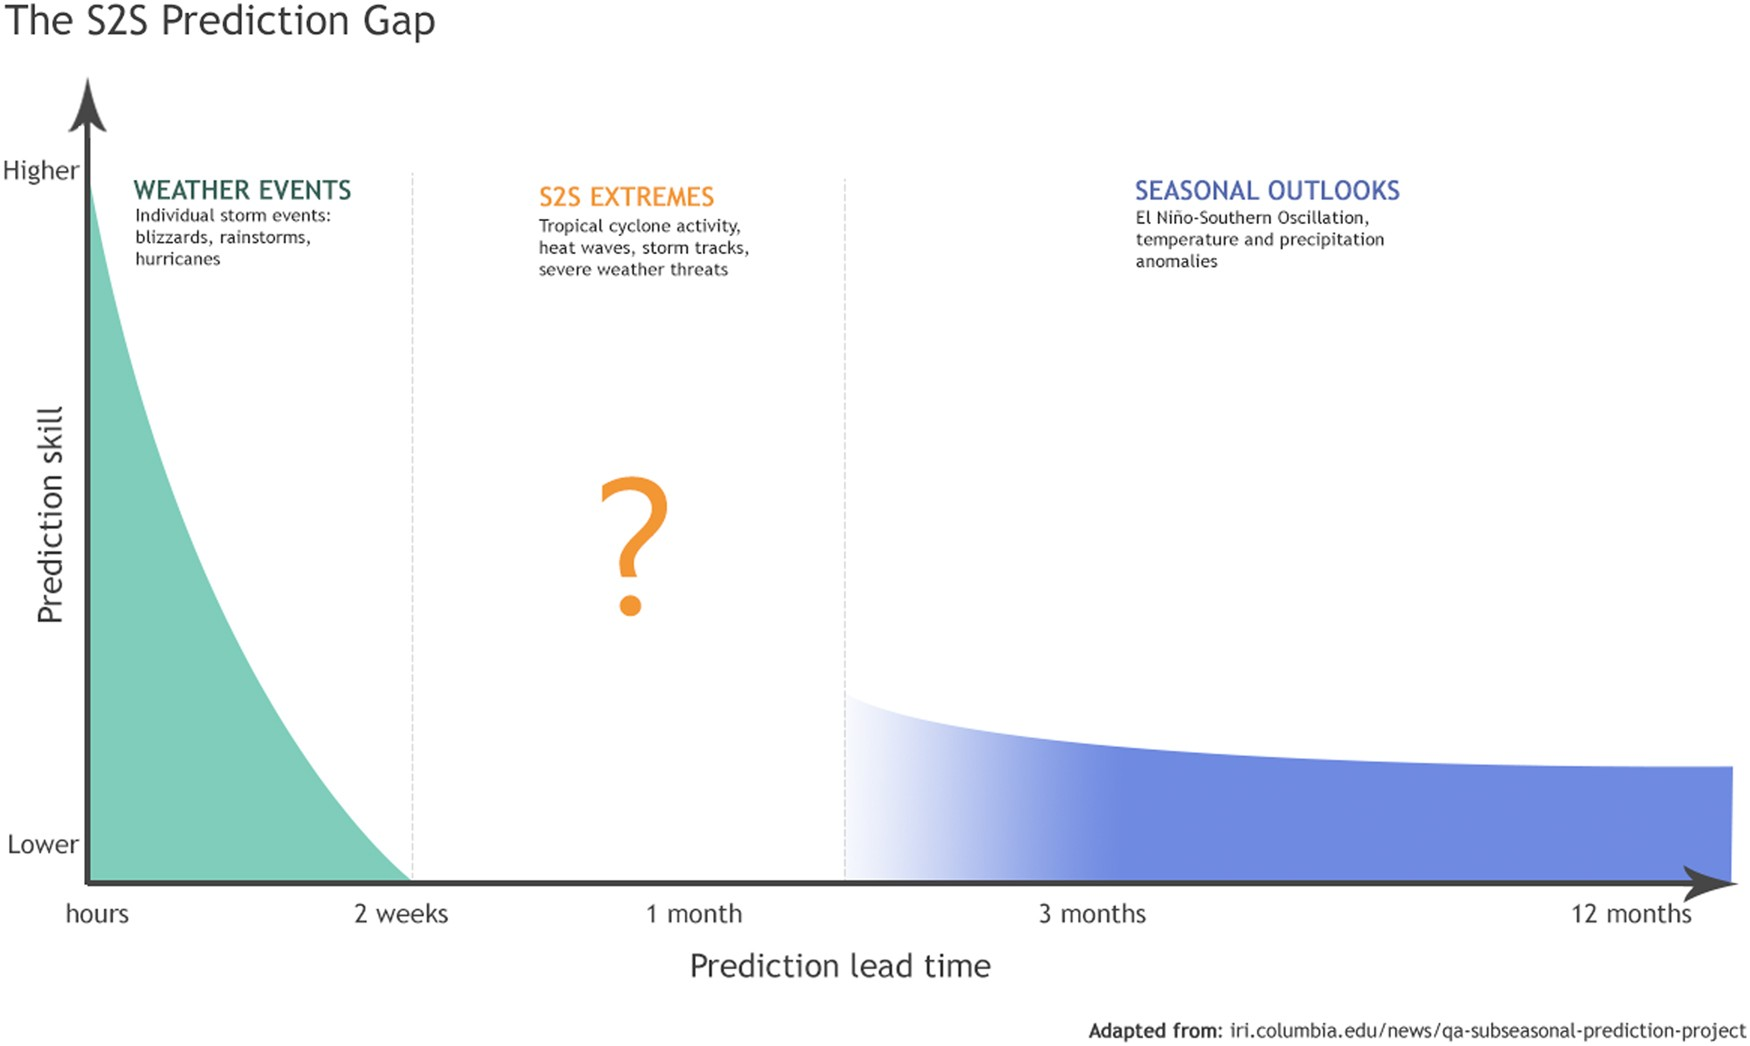
\includegraphics[width=\textwidth, keepaspectratio,
                trim=0 30 0 0, clip]
                {s2s_prediction_gap_mariotti2018.jpg}\\[-0.2em]
            {\tiny\color{gray!50} Source: Mariotti et al.\ (2018)}
        \end{column}

        \begin{column}{0.26\textwidth}
            \centering
            \vspace{1cm}
            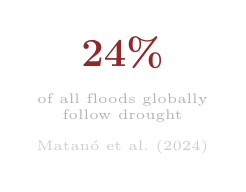
\begin{tikzpicture}
                \node[font=\Large\bfseries, text=gapred!80!black]
                    at (0, 0) {24\%};
                \node[font=\tiny, text=gray!60, align=center]
                    at (0, -0.7) {of all floods globally\\follow drought};
                \node[font=\tiny, text=gray!40]
                    at (0, -1.2) {Matan\'o et al.\ (2024)};
            \end{tikzpicture}
        \end{column}

    \end{columns}

\end{frame}

% SLIDE 2: Literature
\begin{frame}{What Does the Literature Say?}

    \centering
    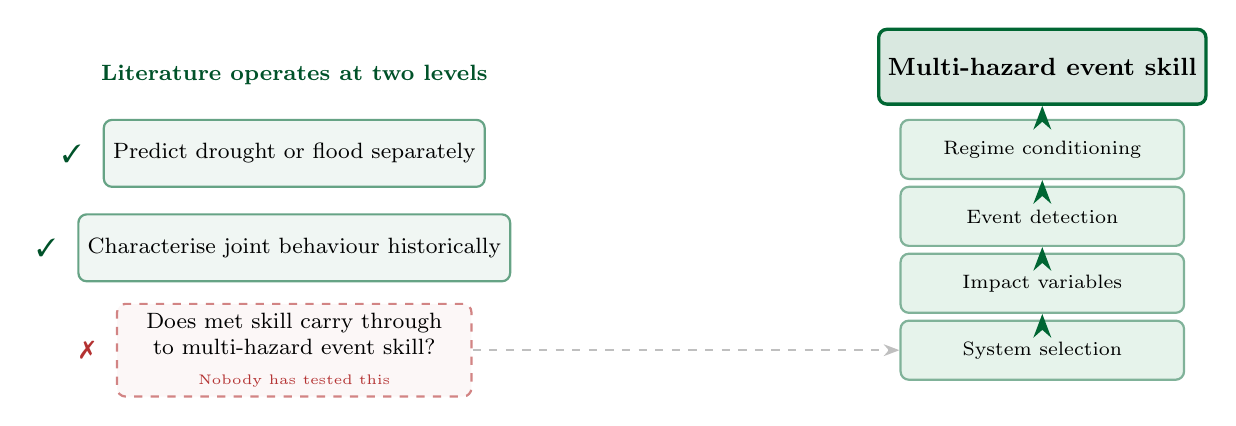
\begin{tikzpicture}[
        level/.style={
            draw=ucdgreen!60, thick, rounded corners=3pt,
            minimum width=4.8cm, minimum height=0.85cm,
            fill=ucdgreen!6, align=center, font=\footnotesize
        },
        levelgap/.style={
            draw=gapred!60, thick, rounded corners=3pt, dashed,
            minimum width=4.8cm, minimum height=0.85cm,
            fill=gapred!4, align=center, font=\footnotesize
        },
        stair/.style={
            draw=ucdgreen!50, thick, rounded corners=3pt,
            minimum width=3.6cm, minimum height=0.75cm,
            fill=stepfill, align=center, font=\scriptsize
        },
        topstair/.style={
            draw=ucdgreen, very thick, rounded corners=3pt,
            minimum width=3.6cm, minimum height=0.75cm,
            fill=topfill!15, align=center, font=\scriptsize\bfseries
        },
        tick/.style={font=\small, text=ucdgreen!80!black},
        cross/.style={font=\small, text=gapred},
        arr/.style={-{Stealth[length=2mm]}, thick, gray!50}
    ]

    % === LEFT: Three levels ===
    \node[font=\footnotesize\bfseries, text=ucdgreen!80!black]
        at (-5.0, 2.8) {Literature operates at two levels};

    \node[level, minimum width=4.5cm] (l1) at (-5.0, 1.8)
        {Predict drought or flood separately};
    \node[tick, left=0.15cm of l1] {\ding{51}};

    \node[level, minimum width=4.5cm] (l2) at (-5.0, 0.6)
        {Characterise joint behaviour historically};
    \node[tick, left=0.15cm of l2] {\ding{51}};

    \node[levelgap, minimum width=4.5cm, minimum height=1.1cm] (l3) at (-5.0, -0.7)
        {Does met skill carry through\\to multi-hazard event skill?\\[0.15em]
         {\tiny\color{gapred} Nobody has tested this}};
    \node[cross, left=0.15cm of l3] {\ding{55}};

    % === RIGHT: Staircase ===
    \node[font=\footnotesize\bfseries, text=ucdgreen!80!black]
        at (4.5, 2.8) {What must be built};

    \node[stair] (s1) at (4.5, -0.7)
        {System selection};

    \draw[-{Stealth[length=2mm]}, thick, gray!50, dashed]
        (l3.east) -- (s1.west);

    \node[stair] (s2) at (4.5, 0.15)
        {Impact variables};
    \draw[-{Stealth[length=3mm]}, very thick, ucdgreen]
        (s1.north) -- (s2.south);

    \node[stair] (s3) at (4.5, 1.0)
        {Event detection};
    \draw[-{Stealth[length=3mm]}, very thick, ucdgreen]
        (s2.north) -- (s3.south);

    \node[stair] (s4) at (4.5, 1.85)
        {Regime conditioning};
    \draw[-{Stealth[length=3mm]}, very thick, ucdgreen]
        (s3.north) -- (s4.south);

    \node[topstair, minimum height=0.95cm, minimum width=4.0cm,
          font=\small\bfseries] (s5) at (4.5, 2.9)
        {Multi-hazard event skill};
    \draw[-{Stealth[length=3mm]}, very thick, ucdgreen]
        (s4.north) -- (s5.south);

    \end{tikzpicture}

\end{frame}

% SLIDE 3: Research Arc
\begin{frame}{Research Arc}

    \vspace{0.3em}
    \begin{enumerate}
        \item[\textcolor{ucdgreen}{\textbf{1.}}] {\itshape How does prediction skill at S2S lead times compare across forecast variables, impact variables, and multi-hazard events?}
        \item[\textcolor{ucdgreen}{\textbf{2.}}] {\itshape Under what atmospheric conditions does this skill emerge?}
    \end{enumerate}

    \vspace{0.6em}

    \centering
    
\begin{tikzpicture}[
        pbox/.style={draw=ucdgreen!40, thick, rounded corners=4pt,
            minimum width=4.0cm, minimum height=1.2cm,
            fill=ucdgreen!5, align=center, font=\footnotesize}
    ]
    \node[pbox, fill=donefill, draw=ucdgreen!60] (pa) at (0, 0)
        {\textbf{Paper 1}\\[0.15em]
         {\scriptsize Drought-to-flood}\\[-0.1em]
         {\tiny\color{ucdgreen!70!black} temporally compounding}};
    \node[pbox, fill=nextfill, draw=orange!50] (pb) at (4.8, 0)
        {\textbf{Paper 2}\\[0.15em]
         {\scriptsize RES droughts}\\[-0.1em]
         {\tiny\color{orange!70!black} multivariate}};
    \node[pbox, fill=gray!8, draw=gray!40] (pc) at (9.6, 0)
        {\textbf{Paper 3}\\[0.15em]
         {\scriptsize ANTICIPATE COST Action}\\[-0.1em]
         {\tiny\color{gray} to be determined}};
    \end{tikzpicture}

    \vspace{1.2em}

    \centering
    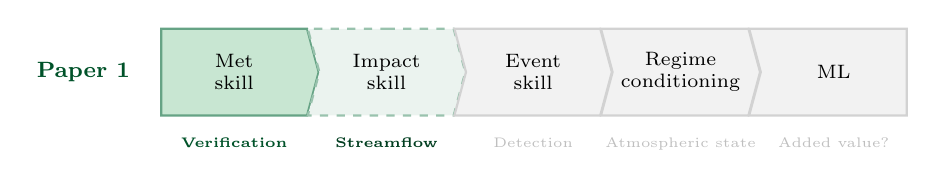
\begin{tikzpicture}[
        xscale=1.0,
        chev/.style={
            minimum width=2.0cm, minimum height=1.1cm,
            align=center, font=\scriptsize, inner sep=3pt,
            signal, signal to=east, signal from=west,
            signal pointer angle=150,
            thick
        },
        plbl/.style={font=\tiny, below=0.15cm}
    ]

    \node[font=\footnotesize\bfseries, text=ucdgreen!80!black,
          anchor=east] at (-1.2, 0) {Paper 1};

    \node[chev, fill=donefill, draw=ucdgreen!60,
          signal from=none] (p1) at (0, 0)
        {Met\\skill};
    \node[plbl, text=ucdgreen!80!black, font=\tiny\bfseries]
        at (p1.south) {Verification};

    \node[chev, fill=ucdgreen!8, draw=ucdgreen!40, dashed,
          right=-0.02cm of p1] (p2)
        {Impact\\skill};
    \node[plbl, text=ucdgreen!60!black, font=\tiny\bfseries]
        at (p2.south) {Streamflow};

    \node[chev, fill=gray!10, draw=gray!35,
          right=-0.02cm of p2] (p3)
        {Event\\skill};
    \node[plbl, text=gray!50]
        at (p3.south) {Detection};

    \node[chev, fill=gray!10, draw=gray!35,
          right=-0.02cm of p3] (p4)
        {Regime\\conditioning};
    \node[plbl, text=gray!50]
        at (p4.south) {Atmospheric state};

    \node[chev, fill=gray!10, draw=gray!35,
          signal to=none, right=-0.02cm of p4] (p6)
        {ML};
    \node[plbl, text=gray!50]
        at (p6.south) {Added value?};

    \end{tikzpicture}

\end{frame}

% SLIDE 4: System comparison
\begin{frame}{Subseasonal vs Seasonal}

    \begin{columns}[c, totalwidth=\textwidth]

        \begin{column}{0.42\textwidth}

            \vspace{-0.5em}
            \centering
            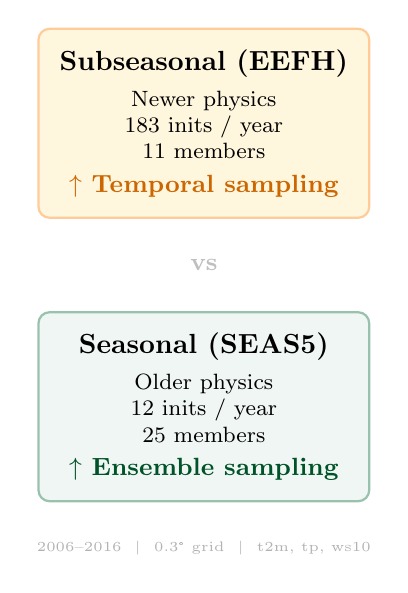
\begin{tikzpicture}[
                sysbox/.style={draw=ucdgreen!40, thick, rounded corners=4pt,
                    minimum width=4.2cm, minimum height=2.4cm,
                    fill=ucdgreen!4, align=center, font=\footnotesize}
            ]
            \node[sysbox, fill=nextfill!60, draw=orange!40] (eefh) at (0, 1.8)
                {\textbf{\normalsize Subseasonal (EEFH)}\\[0.4em]
                 Newer physics\\
                 183 inits / year\\
                 11 members\\[0.3em]
                 {\small\bfseries\color{orange!80!black} $\uparrow$ Temporal sampling}};

            \node[sysbox, fill=ucdgreen!6, draw=ucdgreen!40] (seas) at (0, -1.8)
                {\textbf{\normalsize Seasonal (SEAS5)}\\[0.4em]
                 Older physics\\
                 12 inits / year\\
                 25 members\\[0.3em]
                 {\small\bfseries\color{ucdgreen!80!black} $\uparrow$ Ensemble sampling}};

            \node[font=\small\bfseries, text=gray!50] at (0, 0) {vs};

            \node[font=\tiny, text=gray!60, align=center] at (0, -3.6)
                {2006--2016 ~\textbar~ 0.3\textdegree{} grid ~\textbar~ t2m, tp, ws10};

            \end{tikzpicture}

        \end{column}

        \begin{column}{0.56\textwidth}
            \centering
            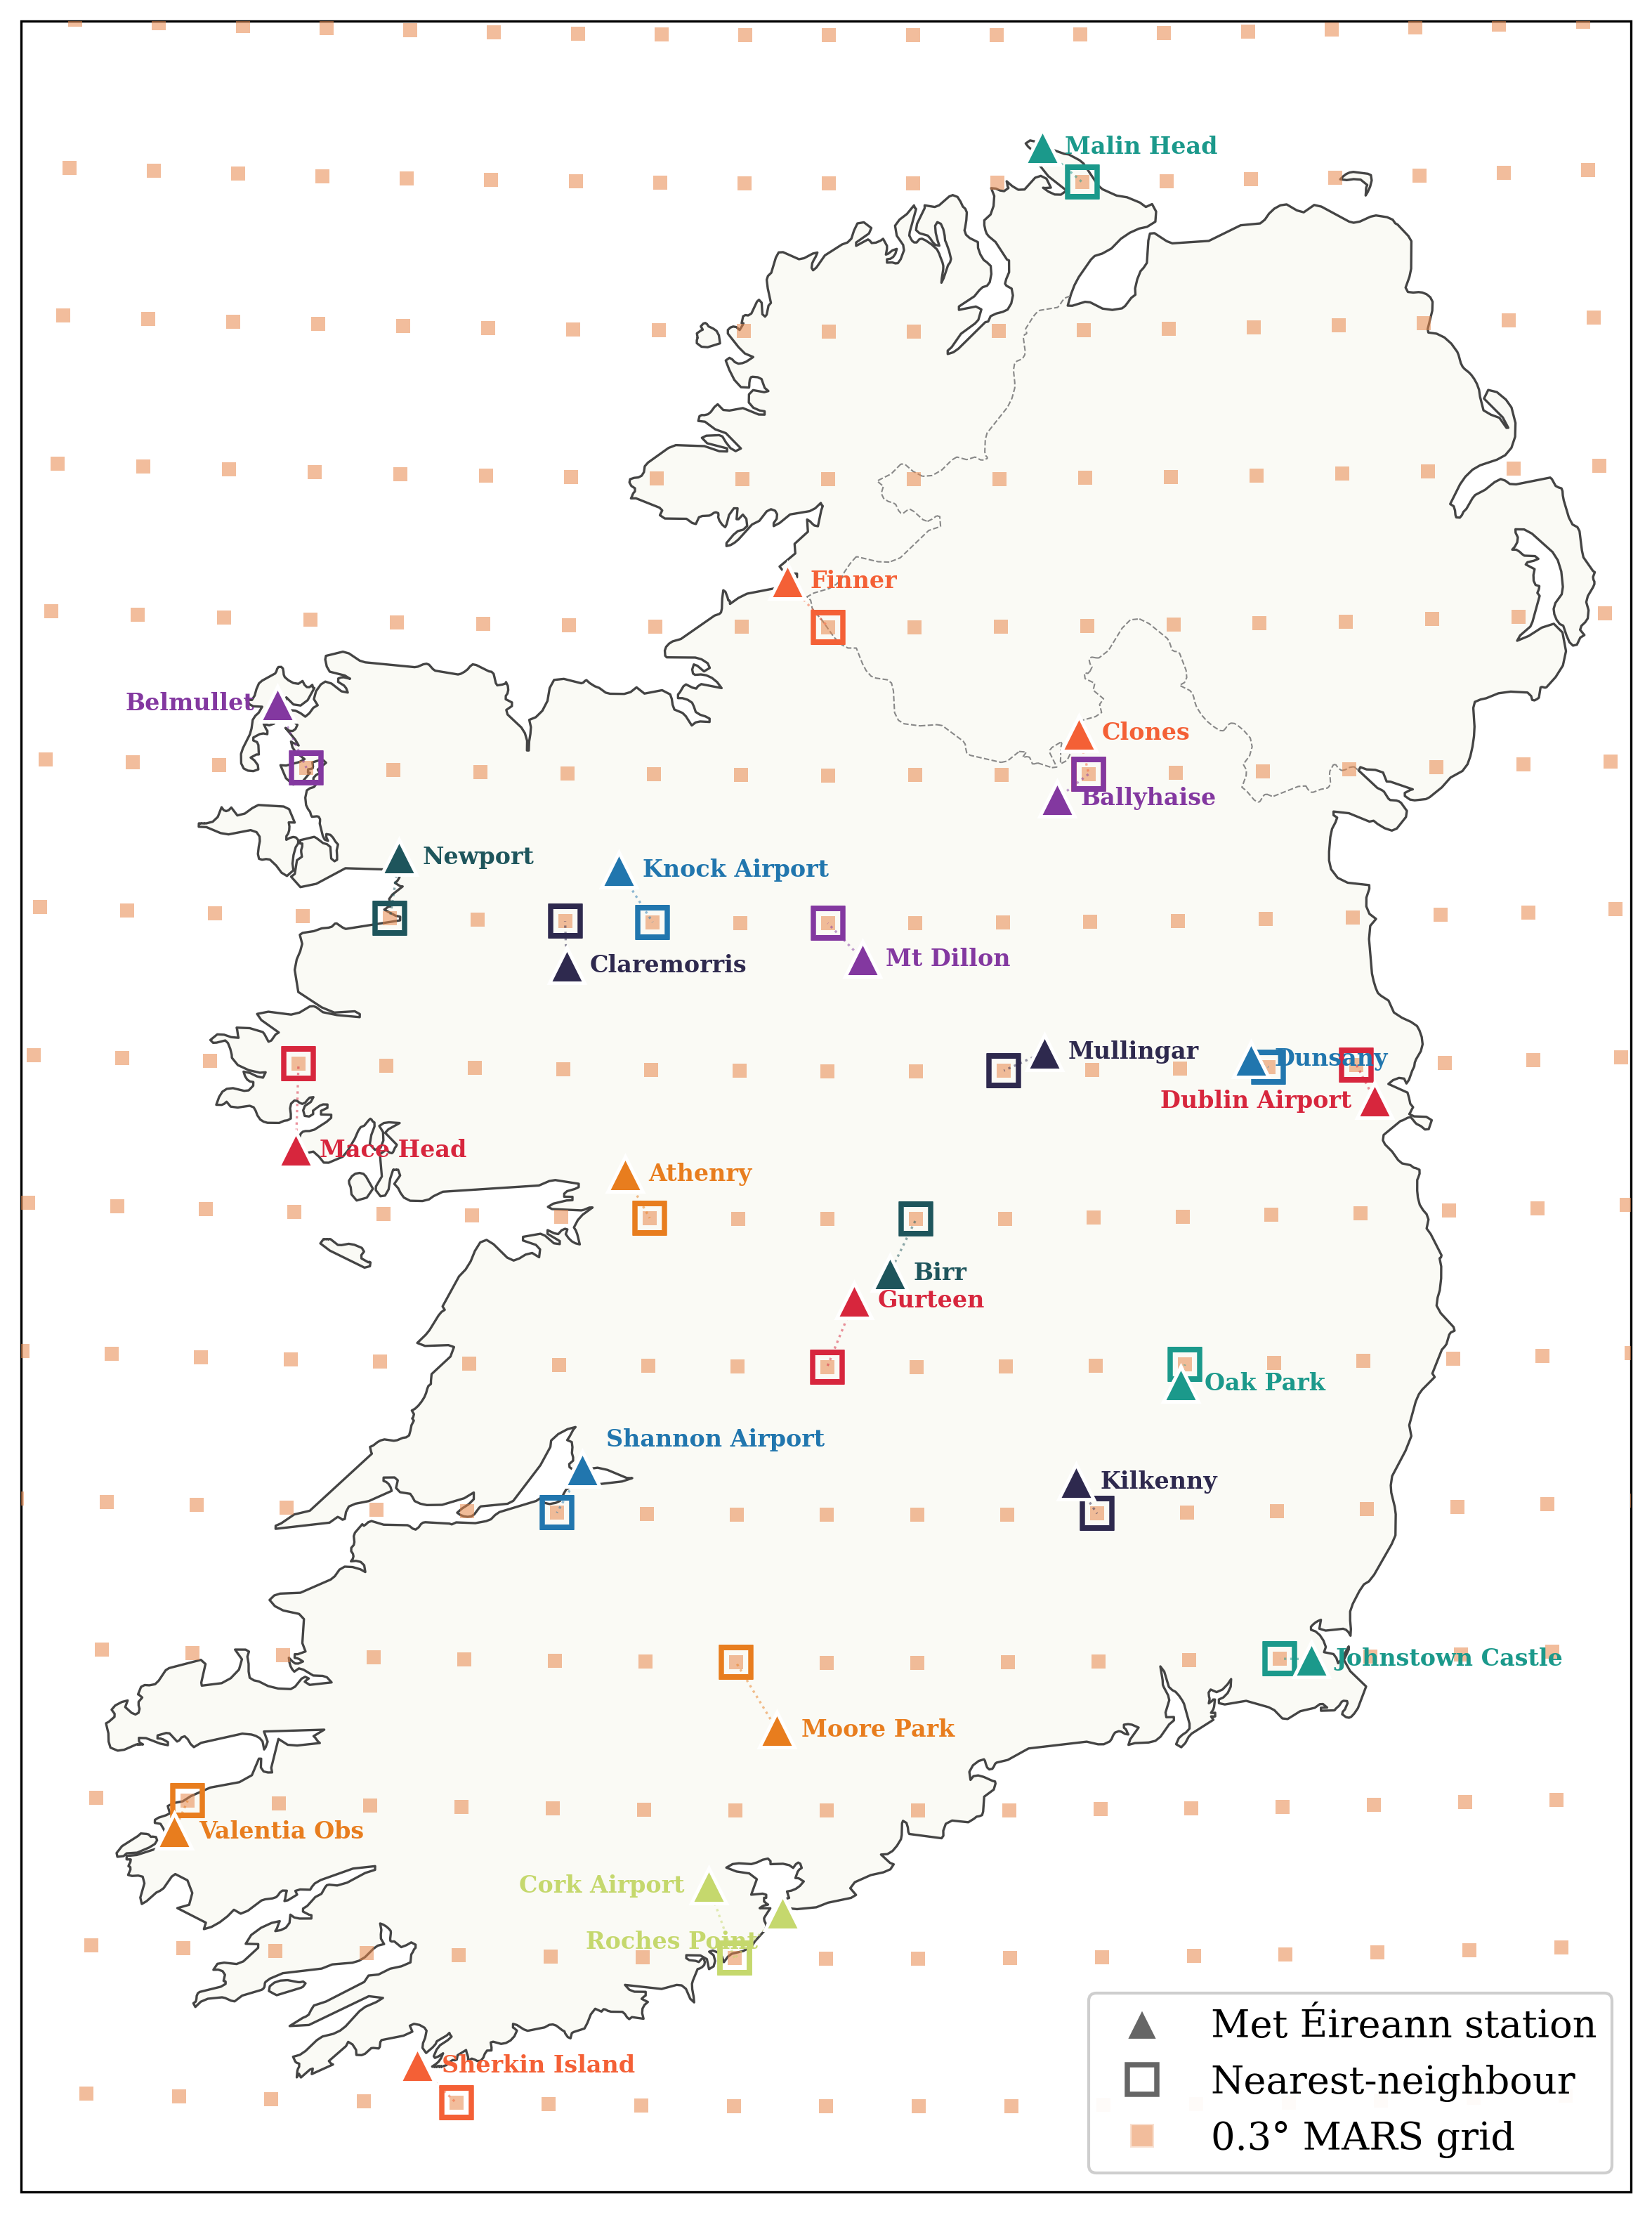
\includegraphics[width=\textwidth, height=0.85\textheight, keepaspectratio]{station_pipeline_nn_map.png}
        \end{column}

    \end{columns}

\end{frame}

% SLIDE 4b: Raw t2m chain
\begin{frame}{Observation--Forecast Temperature Chain}

    \begin{columns}[c, totalwidth=\textwidth]

        \begin{column}{\textwidth}
            \centering
            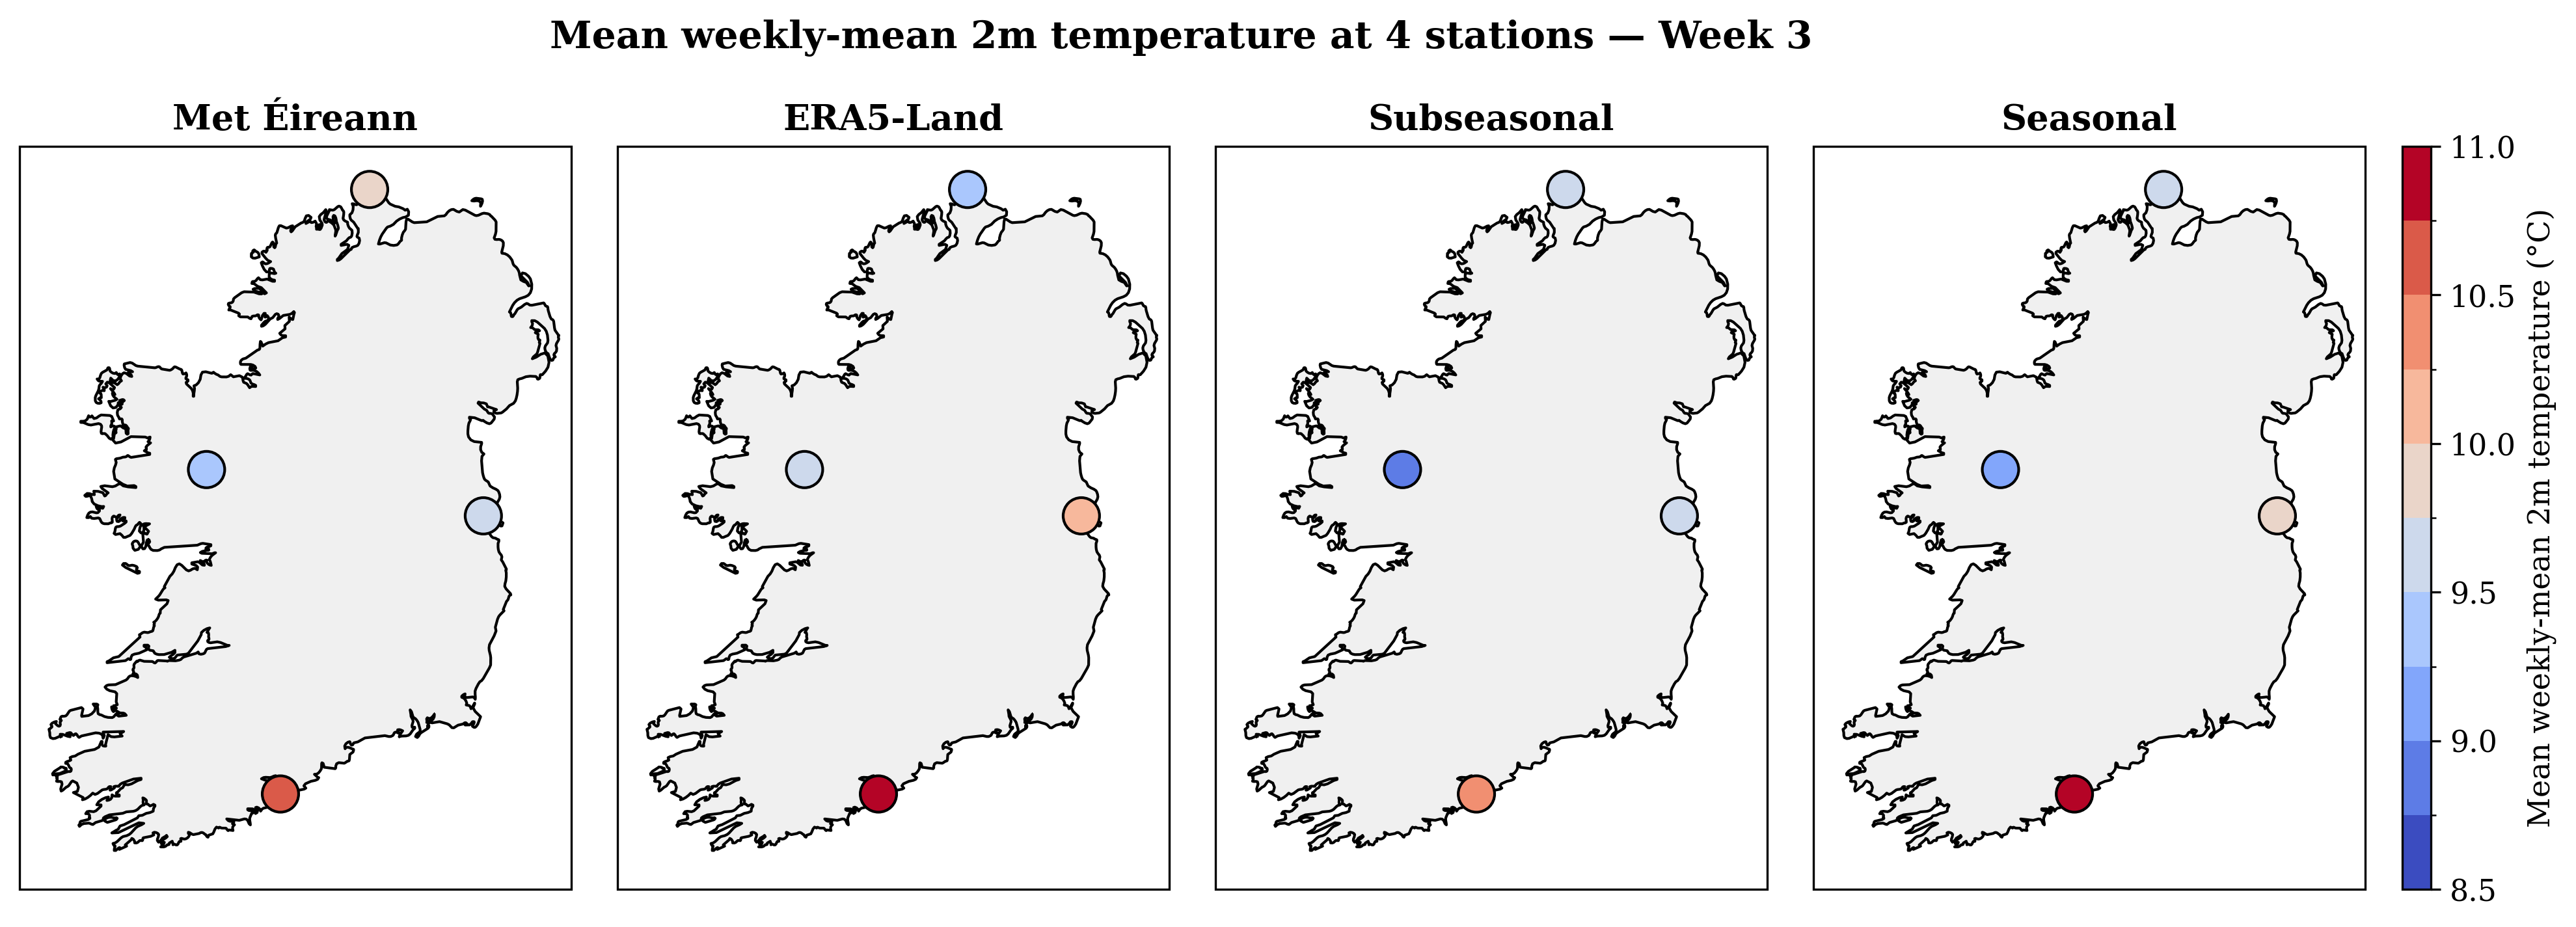
\includegraphics[width=\textwidth, height=0.75\textheight, keepaspectratio]{consolidation_raw_t2m_chain.png}
        \end{column}

    \end{columns}

    \vspace{0.3em}
    
\begin{tikzpicture}
        \node[font=\scriptsize, text=gray!70, anchor=west] at (0, 0)
            {1.~ERA5-Land warm-biased relative to stations};
        \node[font=\scriptsize, text=gray!70, anchor=west] at (7, 0)
            {2.~Seasonal warmer than subseasonal};
    \end{tikzpicture}

\end{frame}

% SLIDE 5: Spatial Bias
\begin{frame}{Spatial Verification}

    \begin{columns}[c, totalwidth=\textwidth]

        \begin{column}{\textwidth}
            \centering
            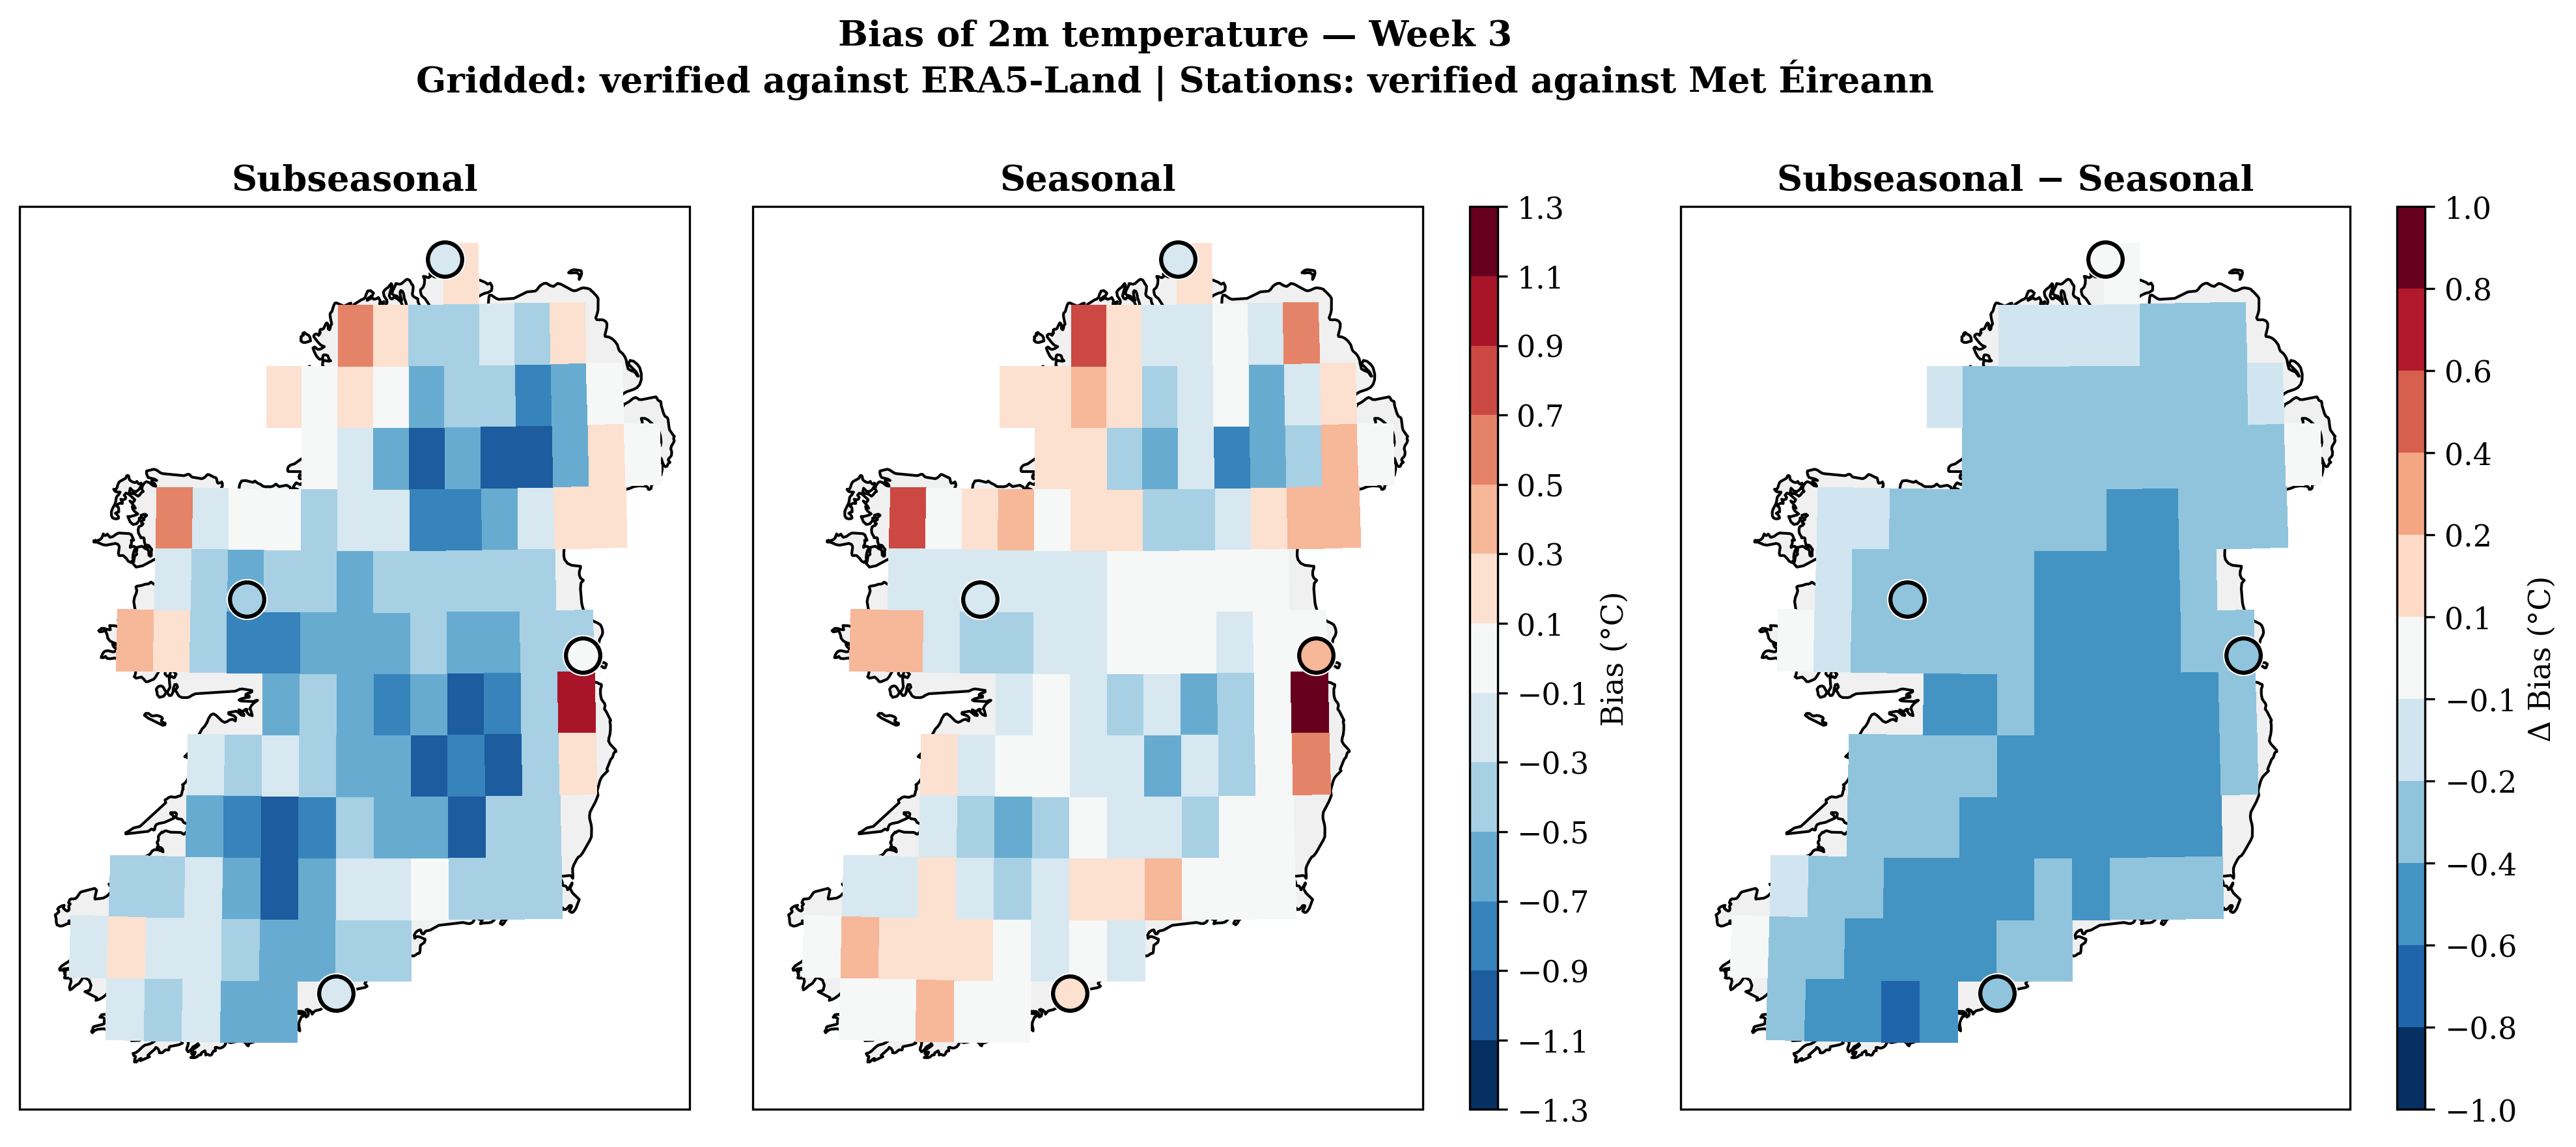
\includegraphics[width=\textwidth, height=0.75\textheight, keepaspectratio]{consolidation_spatial_bias_4panel.png}
        \end{column}

    \end{columns}

    \vspace{0.3em}
    
\begin{tikzpicture}
        \node[font=\scriptsize, text=gray!70, anchor=west] at (0, 0)
            {1.~Subseasonal cold bias exaggerated by warm reference};
        \node[font=\scriptsize, text=gray!70, anchor=west] at (7.5, 0)
            {2.~Seasonal warm bias is genuine};
    \end{tikzpicture}

\end{frame}

% SLIDE 6: Training & Development
\begin{frame}{Training \& Development}

    % --- Credits pill bar ---
    \vspace{0.2em}
    
\begin{tikzpicture}
        \node[font=\footnotesize\bfseries, text=ucdgreen!80!black,
              anchor=west] at (0, 0) {Credits};
        \fill[ucdgreen!35, rounded corners=3pt]
            (1.8, -0.25) rectangle (3.8, 0.25);
        \node[font=\tiny, text=ucdgreen!90!black] at (2.8, 0)
            {ACM41070 (5)};
        \fill[ucdgreen!35, rounded corners=3pt]
            (3.95, -0.25) rectangle (5.95, 0.25);
        \node[font=\tiny, text=ucdgreen!90!black] at (4.95, 0)
            {STAT41130 (5)};
        \fill[nextfill, rounded corners=3pt, draw=orange!40]
            (6.1, -0.25) rectangle (8.1, 0.25);
        \node[font=\tiny, text=orange!80!black] at (7.1, 0)
            {COMP41850 (5)};
        \fill[gray!25, rounded corners=3pt]
            (8.25, -0.25) rectangle (9.75, 0.25);
        \node[font=\tiny, text=gray!70] at (9.0, 0)
            {RPL (15)};
    \end{tikzpicture}

    \vspace{0.3em}

    % --- Training pill bar ---
    
\begin{tikzpicture}
        \node[font=\footnotesize\bfseries, text=ucdgreen!80!black,
              anchor=west] at (0, 0) {Training};
        \fill[ucdgreen!25, rounded corners=3pt]
            (1.8, -0.25) rectangle (4.2, 0.25);
        \node[font=\tiny, text=ucdgreen!90!black] at (3.0, 0)
            {Research integrity};
        \fill[ucdgreen!25, rounded corners=3pt]
            (4.35, -0.25) rectangle (5.95, 0.25);
        \node[font=\tiny, text=ucdgreen!90!black] at (5.15, 0)
            {HPC};
        \fill[ucdgreen!25, rounded corners=3pt]
            (6.1, -0.25) rectangle (8.3, 0.25);
        \node[font=\tiny, text=ucdgreen!90!black] at (7.2, 0)
            {Ark presentation};
        \fill[nextfill, rounded corners=3pt, draw=orange!40]
            (8.45, -0.25) rectangle (10.55, 0.25);
        \node[font=\tiny, text=orange!80!black] at (9.5, 0)
            {DestinE ML};
    \end{tikzpicture}

    \vspace{0.5em}

    % --- Timeline ---
    \centering
    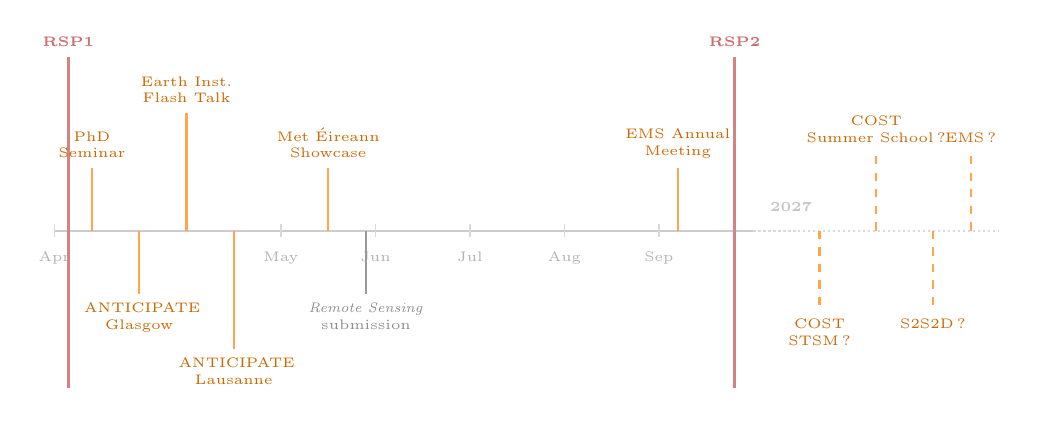
\begin{tikzpicture}[
        xscale=1.2,
        evt/.style={font=\tiny, align=center, text width=2.2cm},
        lbl/.style={font=\tiny, text=gray!60}
    ]

    \draw[thick, gray!40] (0, 0) -- (7.4, 0);
    \draw[thick, gray!30, densely dotted] (7.4, 0) -- (10.0, 0);

    \foreach \x/\m in {
        0.0/Apr, 2.4/May, 3.4/Jun, 4.4/Jul, 5.4/Aug, 6.4/Sep}
    {
        \draw[gray!30] (\x, -0.08) -- (\x, 0.08);
        \node[lbl, below=2pt] at (\x, -0.08) {\m};
    }

    \draw[gapred!60, thick] (0.15, -2.0) -- (0.15, 2.2);
    \node[font=\tiny\bfseries, text=gapred!70] at (0.15, 2.4) {RSP1};

    \draw[gapred!60, thick] (7.2, -2.0) -- (7.2, 2.2);
    \node[font=\tiny\bfseries, text=gapred!70] at (7.2, 2.4) {RSP2};

    \draw[orange!70, thick] (0.4, 0) -- (0.4, 0.8);
    \node[evt, text=orange!80!black, above, text width=1.4cm] at (0.4, 0.8) {PhD\\Seminar};

    \draw[orange!70, thick] (0.9, 0) -- (0.9, -0.8);
    \node[evt, text=orange!80!black, below, text width=1.4cm] at (0.9, -0.8) {ANTICIPATE\\Glasgow};

    \draw[orange!70, thick] (1.4, 0) -- (1.4, 1.5);
    \node[evt, text=orange!80!black, above, text width=1.4cm] at (1.4, 1.5) {Earth Inst.\\Flash Talk};

    \draw[orange!70, thick] (1.9, 0) -- (1.9, -1.5);
    \node[evt, text=orange!80!black, below, text width=1.4cm] at (1.9, -1.5) {ANTICIPATE\\Lausanne};

    \draw[orange!70, thick] (2.9, 0) -- (2.9, 0.8);
    \node[evt, text=orange!80!black, above, text width=1.8cm] at (2.9, 0.8) {Met \'Eireann\\Showcase};

    \draw[gray!80, thick] (3.3, 0) -- (3.3, -0.8);
    \node[evt, text=gray!90, below, text width=1.8cm] at (3.3, -0.8) {\textit{Remote Sensing}\\submission};

    \draw[orange!70, thick] (6.6, 0) -- (6.6, 0.8);
    \node[evt, text=orange!80!black, above] at (6.6, 0.8) {EMS Annual\\Meeting};

    \node[font=\tiny\bfseries, text=gray!45] at (7.8, 0.3) {2027};

    \draw[orange!70, thick, dashed] (8.1, 0) -- (8.1, -1.0);
    \node[evt, text=orange!80!black, below, text width=1.8cm] at (8.1, -1.0) {COST\\STSM\,?};

    \draw[orange!70, thick, dashed] (8.7, 0) -- (8.7, 1.0);
    \node[evt, text=orange!80!black, above, text width=1.8cm] at (8.7, 1.0) {COST\\Summer School\,?};

    \draw[orange!70, thick, dashed] (9.3, 0) -- (9.3, -1.0);
    \node[evt, text=orange!80!black, below, text width=1.6cm] at (9.3, -1.0) {S2S2D\,?};

    \draw[orange!70, thick, dashed] (9.7, 0) -- (9.7, 1.0);
    \node[evt, text=orange!80!black, above, text width=1.4cm] at (9.7, 1.0) {EMS\,?};

    \end{tikzpicture}

\end{frame}

% References
\begin{frame}{References}

    \scriptsize
    \begin{itemize}\setlength{\itemsep}{0.45em}

    \item Anderson, B.~J., and Coauthors, 2025: What is a drought-to-flood transition? Pitfalls and recommendations for defining consecutive hydrological extreme events. \textit{Hydrol.\ Earth Syst.\ Sci.}, \textbf{29}, 6069--6092.

    \item DeFlorio, M.~J., and Coauthors, 2024: From California's extreme drought to major flooding: Evaluating and synthesizing experimental seasonal and subseasonal forecasts during winter 2022/23. \textit{Bull.\ Amer.\ Meteor.\ Soc.}, \textbf{105}, E84--E104.

    \item Dong, N., H.~Hao, M.~Yang, J.~Wei, S.~Xu, and H.~Kunstmann, 2025: Deep-learning-based sub-seasonal precipitation and streamflow ensemble forecasting over the source region of the Yangtze River. \textit{Hydrol.\ Earth Syst.\ Sci.}, \textbf{29}, 2023--2042.

    \item Kratzert, F., D.~Klotz, C.~Brenner, K.~Schulz, and M.~Herrnegger, 2018: Rainfall--runoff modelling using Long Short-Term Memory (LSTM) networks. \textit{Hydrol.\ Earth Syst.\ Sci.}, \textbf{22}, 6005--6022.

    \item Malik, I., and V.~Mishra, 2025: Sub-seasonal prediction of compound hot and dry extremes in India. \textit{Climate Dyn.}, \textbf{63}, 191.

    \item Mariotti, A., and Coauthors, 2020: Windows of opportunity for skillful forecasts subseasonal to seasonal and beyond. \textit{Bull.\ Amer.\ Meteor.\ Soc.}, \textbf{101}, E608--E625.

    \item Rashid, M.~M., and T.~Wahl, 2022: Hydrologic risk from consecutive dry and wet extremes at the global scale. \textit{Environ.\ Res.\ Commun.}, \textbf{4}, 071001.

    \item Zscheischler, J., and Coauthors, 2020: A typology of compound weather and climate events. \textit{Nat.\ Rev.\ Earth Environ.}, \textbf{1}, 333--347.

    \end{itemize}

\end{frame}

% ==========================================================
% BACKUP SLIDES
% ==========================================================
\appendix

% Terminology map (moved here per request)
\begin{frame}{How Do You Detect These Events?}

    \begin{columns}[c, totalwidth=\textwidth]

        \begin{column}{0.75\textwidth}
            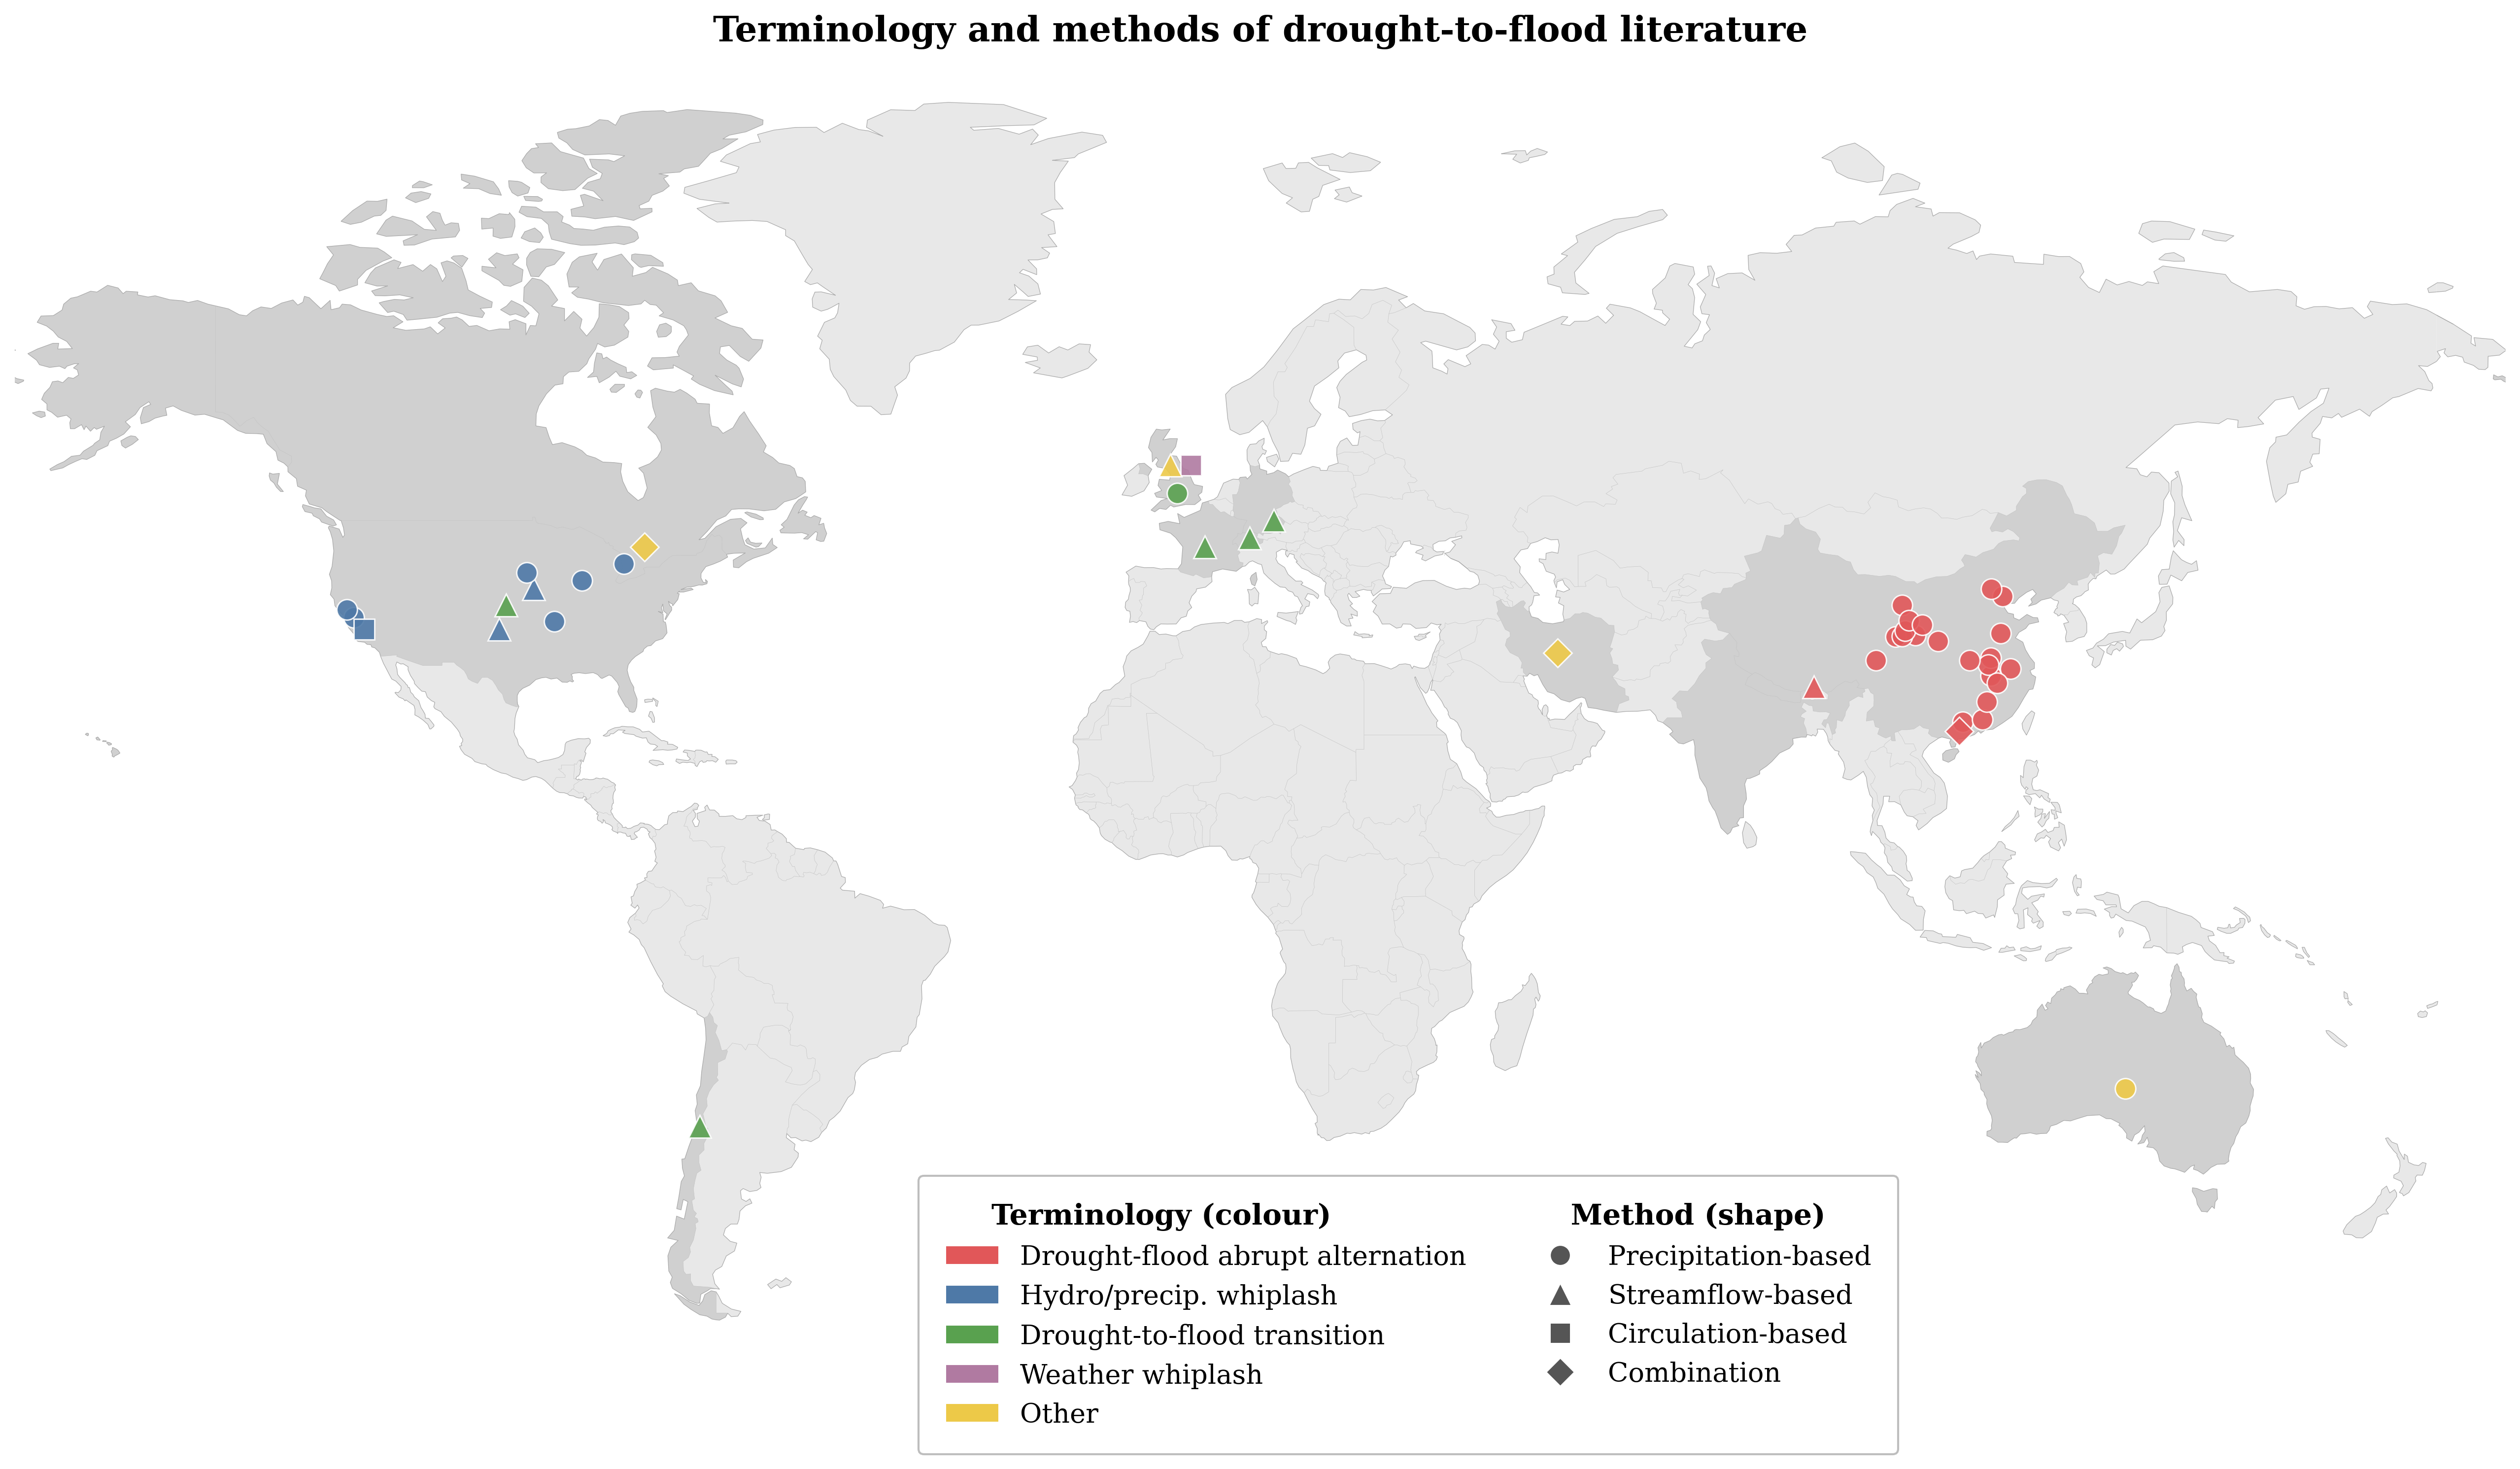
\includegraphics[width=\textwidth]
                {terminology_map.png}
        \end{column}

        \begin{column}{0.23\textwidth}
            \centering
            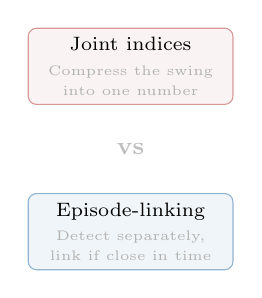
\begin{tikzpicture}[
                vs/.style={font=\small\bfseries, text=gray!50}
            ]

            \node[draw=gapred!50, rounded corners=3pt,
                  minimum width=2.6cm, minimum height=0.9cm,
                  fill=gapred!6, align=center, font=\scriptsize] (ji) at (0, 1.2)
                {Joint indices\\[0.1em]
                 {\tiny\color{gray!60} Compress the swing}\\[-0.1em]
                 {\tiny\color{gray!60} into one number}};

            \node[vs] at (0, 0.15) {vs};

            \node[draw=vennblue!60, rounded corners=3pt,
                  minimum width=2.6cm, minimum height=0.9cm,
                  fill=vennblue!8, align=center, font=\scriptsize] (el) at (0, -0.9)
                {Episode-linking\\[0.1em]
                 {\tiny\color{gray!60} Detect separately,}\\[-0.1em]
                 {\tiny\color{gray!60} link if close in time}};

            \end{tikzpicture}
        \end{column}

    \end{columns}

\end{frame}

% Three strategies (moved here per request)
\begin{frame}{Three strategies for detecting transitions}

    \centering
    \vspace{-0.3em}

    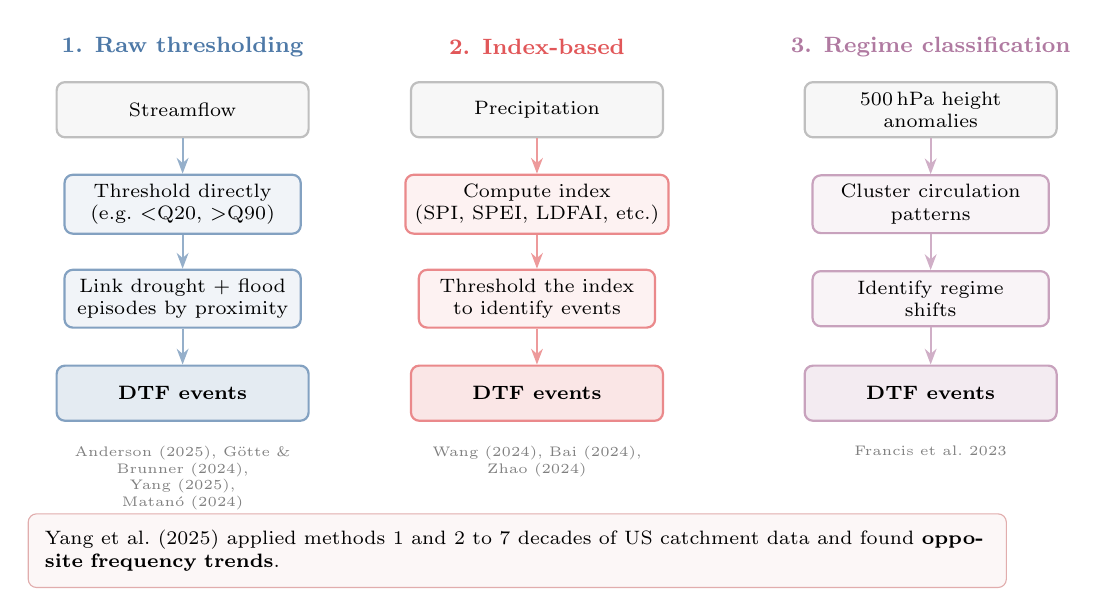
\begin{tikzpicture}[xshift=0.5cm]

    \node[detlbl=strat1] (t1) at (1.0, 3.8) {1. Raw thresholding};
    \node[detdata] (d1) at (1.0, 3.0) {Streamflow};
    \node[detbox=strat1] (th1) at (1.0, 1.8) {Threshold directly\\(e.g.\ $<$Q20, $>$Q90)};
    \node[detbox=strat1] (link1) at (1.0, 0.6) {Link drought + flood\\episodes by proximity};
    \node[detresult=strat1] (ev1) at (1.0, -0.6) {DTF events};

    \draw[detarr=strat1] (d1) -- (th1);
    \draw[detarr=strat1] (th1) -- (link1);
    \draw[detarr=strat1] (link1) -- (ev1);

    \node[font=\tiny, text=gray, anchor=north, text width=3cm, align=center]
        at (1.0, -1.15) {Anderson (2025), G\"otte \&\\Brunner (2024), Yang (2025),\\Matan\'o (2024)};

    \node[detlbl=strat2] (t2) at (5.5, 3.8) {2. Index-based};
    \node[detdata] (d2) at (5.5, 3.0) {Precipitation};
    \node[detbox=strat2] (idx) at (5.5, 1.8) {Compute index\\(SPI, SPEI, LDFAI, etc.)};
    \node[detbox=strat2] (th2) at (5.5, 0.6) {Threshold the index\\to identify events};
    \node[detresult=strat2] (ev2) at (5.5, -0.6) {DTF events};

    \draw[detarr=strat2] (d2) -- (idx);
    \draw[detarr=strat2] (idx) -- (th2);
    \draw[detarr=strat2] (th2) -- (ev2);

    \node[font=\tiny, text=gray, anchor=north, text width=3cm, align=center]
        at (5.5, -1.15) {Wang (2024), Bai (2024),\\Zhao (2024)};

    \node[detlbl=strat3] (t3) at (10.5, 3.8) {3. Regime classification};
    \node[detdata] (d3) at (10.5, 3.0) {500\,hPa height\\anomalies};
    \node[detbox=strat3] (som) at (10.5, 1.8) {Cluster circulation\\patterns};
    \node[detbox=strat3] (shift) at (10.5, 0.6) {Identify regime\\shifts};
    \node[detresult=strat3] (ev3) at (10.5, -0.6) {DTF events};

    \draw[detarr=strat3] (d3) -- (som);
    \draw[detarr=strat3] (som) -- (shift);
    \draw[detarr=strat3] (shift) -- (ev3);

    \node[font=\tiny, text=gray, anchor=north, text width=3cm, align=center]
        at (10.5, -1.15) {Francis et al.\ 2023};

    \node[draw=gapred!40, rounded corners=3pt, fill=gapred!4,
          text width=12cm, align=left, font=\scriptsize, inner sep=6pt]
        at (5.25, -2.6) {
            Yang et al.\ (2025) applied methods 1 and 2 to 7 decades of US catchment data and found \textbf{opposite frequency trends}.
        };

    \end{tikzpicture}

\end{frame}

% Dataset overview
\begin{frame}{Dataset Overview}

    \centering
    \vspace{-0.3em}

    {\footnotesize\textbf{Forecast systems}}
    \vspace{0.3em}

    \footnotesize
    \renewcommand{\arraystretch}{1.3}
    \begin{tabular}{l l l l l l l}
    \toprule
    \textbf{System} & \textbf{Source} & \textbf{IFS cycle} & \textbf{Grid} & \textbf{Members} & \textbf{Reforecast period} & \textbf{Lead range} \\
    \midrule
    Seasonal (SEAS5)       & MARS API & Cy43r1 & 0.28\textdegree{} & 25 & 1981--2016 & 215 days \\
    Subseasonal (EEFH)     & MARS API & Cy49r1 & 0.28\textdegree{} & 11 & 2005--2024 & 46 days  \\
    \bottomrule
    \end{tabular}

    \vspace{0.8em}

    {\footnotesize\textbf{Reference datasets}}
    \vspace{0.3em}

    \footnotesize
    \renewcommand{\arraystretch}{1.3}
    \begin{tabular}{l l l l}
    \toprule
    \textbf{Dataset} & \textbf{Source} & \textbf{Grid} & \textbf{Coverage} \\
    \midrule
    ERA5-Land     & MARS API              & 0.1\textdegree{} & 1950--present \\
    Met \'Eireann & Met \'Eireann archive & Station          & 1945--present (varies by station) \\
    \bottomrule
    \end{tabular}

    \vspace{0.8em}
    \scriptsize
    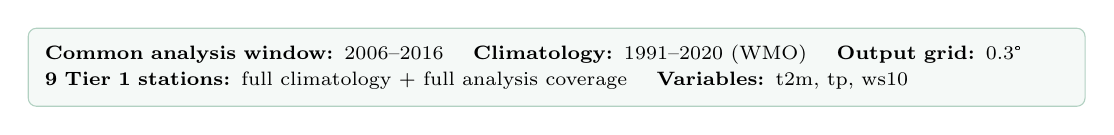
\begin{tikzpicture}
        \node[draw=ucdgreen!30, rounded corners=3pt, fill=ucdgreen!4,
              text width=13cm, align=left, font=\scriptsize, inner sep=6pt] {
            \textbf{Common analysis window:} 2006--2016 \quad
            \textbf{Climatology:} 1991--2020 (WMO) \quad
            \textbf{Output grid:} 0.3\textdegree{} \\[0.2em]
            \textbf{9 Tier~1 stations:} full climatology + full analysis coverage \quad
            \textbf{Variables:} t2m, tp, ws10
        };
    \end{tikzpicture}

\end{frame}

% System comparison table
\begin{frame}{Subseasonal vs Seasonal: System Comparison}

    \centering
    \vspace{-0.3em}

    \footnotesize
    \renewcommand{\arraystretch}{1.4}
    \begin{tabular}{l c c}
    \toprule
     & \textbf{Subseasonal (EEFH)} & \textbf{Seasonal (SEAS5)} \\
    \midrule
    IFS cycle            & Cy49r1 (2024)       & Cy43r1 (2016) \\
    Grid type            & Cubic octahedral     & Reduced Gaussian \\
    Resolution           & $\sim$32 km (TCo319) & $\sim$36 km (T319) \\
    Vertical levels      & 137                  & 91 \\
    Stochastic physics   & SPP (27 parameters)  & SPPT3 + SKEB \\
    Ozone--radiation     & Fully interactive    & Climatological \\
    Reforecast members   & 11                   & 25 \\
    Real-time members    & 101                  & 51 \\
    Init frequency       & Every odd day        & 1st of month \\
    Reforecast period    & Prior 20 yr (rolling) & 1981--2016 (fixed) \\
    Lead range           & 46 days              & 215 days \\
    Atm.\ initial conds  & ERA5                 & ERA-Interim \\
    \bottomrule
    \end{tabular}

    \vspace{0.8em}
    \scriptsize
    
\begin{tikzpicture}
        \node[draw=ucdgreen!30, rounded corners=3pt, fill=ucdgreen!4,
              text width=12cm, align=left, font=\scriptsize, inner sep=6pt] {
            \textbf{Matched comparison:} 2006--2016, 1st-of-month inits, 0.3\textdegree{} grid over Ireland. \\
            Differences then reflect \textbf{model physics and ensemble size}, not data coverage.
        };
    \end{tikzpicture}

\end{frame}

% Three research traditions
\begin{frame}{Three research traditions}

    \centering
    \vspace{-0.3em}

    \footnotesize
    \renewcommand{\arraystretch}{1.4}
    \begin{tabular}{l l l l}
    \toprule
     & \textbf{DFAA} & \textbf{Western whiplash / transition} & \textbf{Weather whiplash} \\
    \midrule
    Origin          & Chinese hydrology          & US and Europe                          & Atmospheric science \\
    Primary variable & Precipitation (SPI-based)  & Precipitation, streamflow, or both     & 500\,hPa geopotential height \\
    Detection logic  & Purpose-built alternation   & Independent episode detection,         & Regime classification \\
                     & indices (single scalar)     & linked by temporal proximity           & via self-organising maps \\
    Seasonality      & Monsoon-specific            & Various                                & Synoptic timescales \\
    Research focus   & Characterisation            & Trends and prediction                  & Regime dynamics \\
    Role of ML       & None                        & Emerging                               & None \\
    \bottomrule
    \end{tabular}

    \vspace{0.8em}
    \scriptsize
    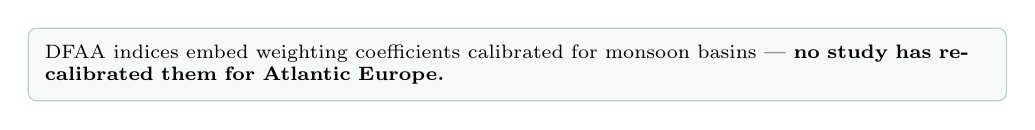
\begin{tikzpicture}
        \node[draw=ucdgreen!30, rounded corners=3pt, fill=ucdgreen!4,
              text width=12cm, align=left, font=\scriptsize, inner sep=6pt] {
            DFAA indices embed weighting coefficients calibrated for monsoon basins ---
            \textbf{no study has recalibrated them for Atlantic Europe.}
        };
    \end{tikzpicture}

\end{frame}

% Event definitions
\begin{frame}{How are drought-to-flood events defined?}

    \centering
    \vspace{-0.5em}

    \scriptsize
    \renewcommand{\arraystretch}{1.25}
    \begin{tabular}{l l c l l l}
    \toprule
    \textbf{Study} & \textbf{Region} & \textbf{Strategy} & \textbf{Drought def.} & \textbf{Flood def.} & \textbf{Transition rule} \\
    \midrule
    G\"otte \&      & US      & 1 & Streamflow $<$ Q20       & Streamflow $>$ Q50       & $\geq$10 days \\
    Brunner (2024)  &         &   & (varies by day-of-year)  & of annual maxima         & \\
    \arrayrulecolor{gray!30}\midrule\arrayrulecolor{black}
    Yang et         & US      & 1 & Streamflow $<$ Q50       & Streamflow $>$ Q50       & $<$90 days \\
    al.\ (2025)     &         &   & of annual 7-day min      & of annual maxima         & \\
    \arrayrulecolor{gray!30}\midrule\arrayrulecolor{black}
    Matan\'o et     & Global  & 1 & $<$Q15 in $\geq$1        & Streamflow               & $<$30 days \\
    al.\ (2024)     &         &   & hydrological variable    & $>$ Q85                  & \\
    \arrayrulecolor{gray!30}\midrule\arrayrulecolor{black}
    Guimar\~aes     & France  & 1 & Streamflow $<$ Q20       & Streamflow $>$ Q99       & No gap \\
    et al.\ (2026)  &         &   &                          &                          & \\
    \arrayrulecolor{gray!30}\midrule\arrayrulecolor{black}
    Wang et         & China   & 2 & SPI $\to$ MSDFAI         & SPI $\to$ MSDFAI         & Index $\geq$ 1 \\
    al.\ (2024)     &         &   & (alternation index)      & (alternation index)      & \\
    \bottomrule
    \end{tabular}

    \vspace{0.8em}
    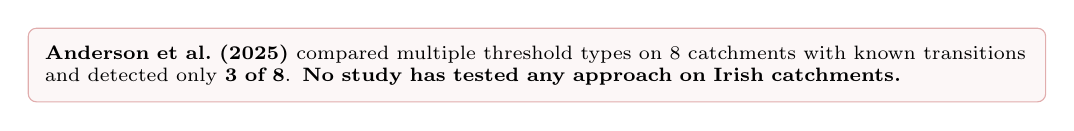
\begin{tikzpicture}
        \node[draw=gapred!40, rounded corners=3pt, fill=gapred!4,
              text width=12.5cm, align=left, font=\scriptsize, inner sep=6pt] {
            \textbf{Anderson et al.\ (2025)} compared multiple threshold types on 8~catchments
            with known transitions and detected only \textbf{3 of 8}.
            \textbf{No study has tested any approach on Irish catchments.}
        };
    \end{tikzpicture}

\end{frame}

% Verification metrics
\begin{frame}{Verification Metrics}

    \vspace{-0.3em}

    {\footnotesize
    $f_i$ = forecast weekly mean, \quad
    $o_i$ = observed weekly mean, \quad
    $\bar{c}_i$ = climatological mean (1991--2020) \\[0.3em]
    $f'_i = f_i - \bar{c}_i$ = forecast anomaly, \quad
    $o'_i = o_i - \bar{c}_i$ = observed anomaly, \quad
    $N$ = number of cases
    }

    \vspace{0.5em}

    \begin{columns}[T]
    \begin{column}{0.48\textwidth}
        \[
        \mathrm{Bias} = \frac{1}{N}\sum_{i=1}^{N} (f_i - o_i)
        \]

        \[
        \mathrm{RMSE} = \sqrt{\frac{1}{N}\sum_{i=1}^{N} (f_i - o_i)^2}
        \]
    \end{column}

    \begin{column}{0.48\textwidth}
        \[
        \mathrm{ACC} = \frac{\displaystyle\sum_{i} f'_i \, o'_i}
        {\sqrt{\displaystyle\sum_{i} (f'_i)^2} \;\sqrt{\displaystyle\sum_{i} (o'_i)^2}}
        \]

        \vspace{0.3em}
        {\scriptsize
        Uncentred, unweighted, matching the ECMWF operational definition.
        Computed as spatial pattern correlation per init (across gridpoints),
        then averaged across inits.}
    \end{column}
    \end{columns}

\end{frame}

% Pipeline Variables
\begin{frame}{Pipeline Variables}

    \centering

    \footnotesize
    \renewcommand{\arraystretch}{1.4}
    \begin{tabular}{l l l l l l}
    \toprule
    \textbf{Var.} & \textbf{Seasonal} & \textbf{Subseasonal} & \textbf{ERA5-Land} & \textbf{Met \'Eireann} & \textbf{Verif.\ res.} \\
    \midrule
    t2m  & Daily mean      & Daily mean      & Daily mean        & Daily mean    & Daily \\
         & (from 6h inst.) & (from 6h inst.) & (from 6h subset)  & (from hourly) & \\[0.4em]
    tp   & Daily total     & Daily total     & Daily total       & Daily total   & Daily \\
         & (de-accum.\ 6h) & (de-accum.\ 6h) & (from hourly)    & (native)      & \\[0.4em]
    ws10 & Daily mean      & Daily mean      & Daily mean        & Daily mean    & Daily \\
         & (from 6h u10, v10) & (from 6h u10, v10) & (from 6h u10, v10) & (from hourly) & \\
    \bottomrule
    \end{tabular}

    \vspace{1em}
    
\begin{tikzpicture}
        \node[draw=gray!30, rounded corners=3pt, fill=gray!4,
              text width=8cm, align=left, font=\footnotesize, inner sep=6pt] {
            All variables aggregated to \textbf{weekly means} for scoring.
        };
    \end{tikzpicture}

\end{frame}

% Station-level verification
\begin{frame}{Station-Level Verification}

    \begin{columns}[c, totalwidth=\textwidth]

        \begin{column}{\textwidth}
            \centering
            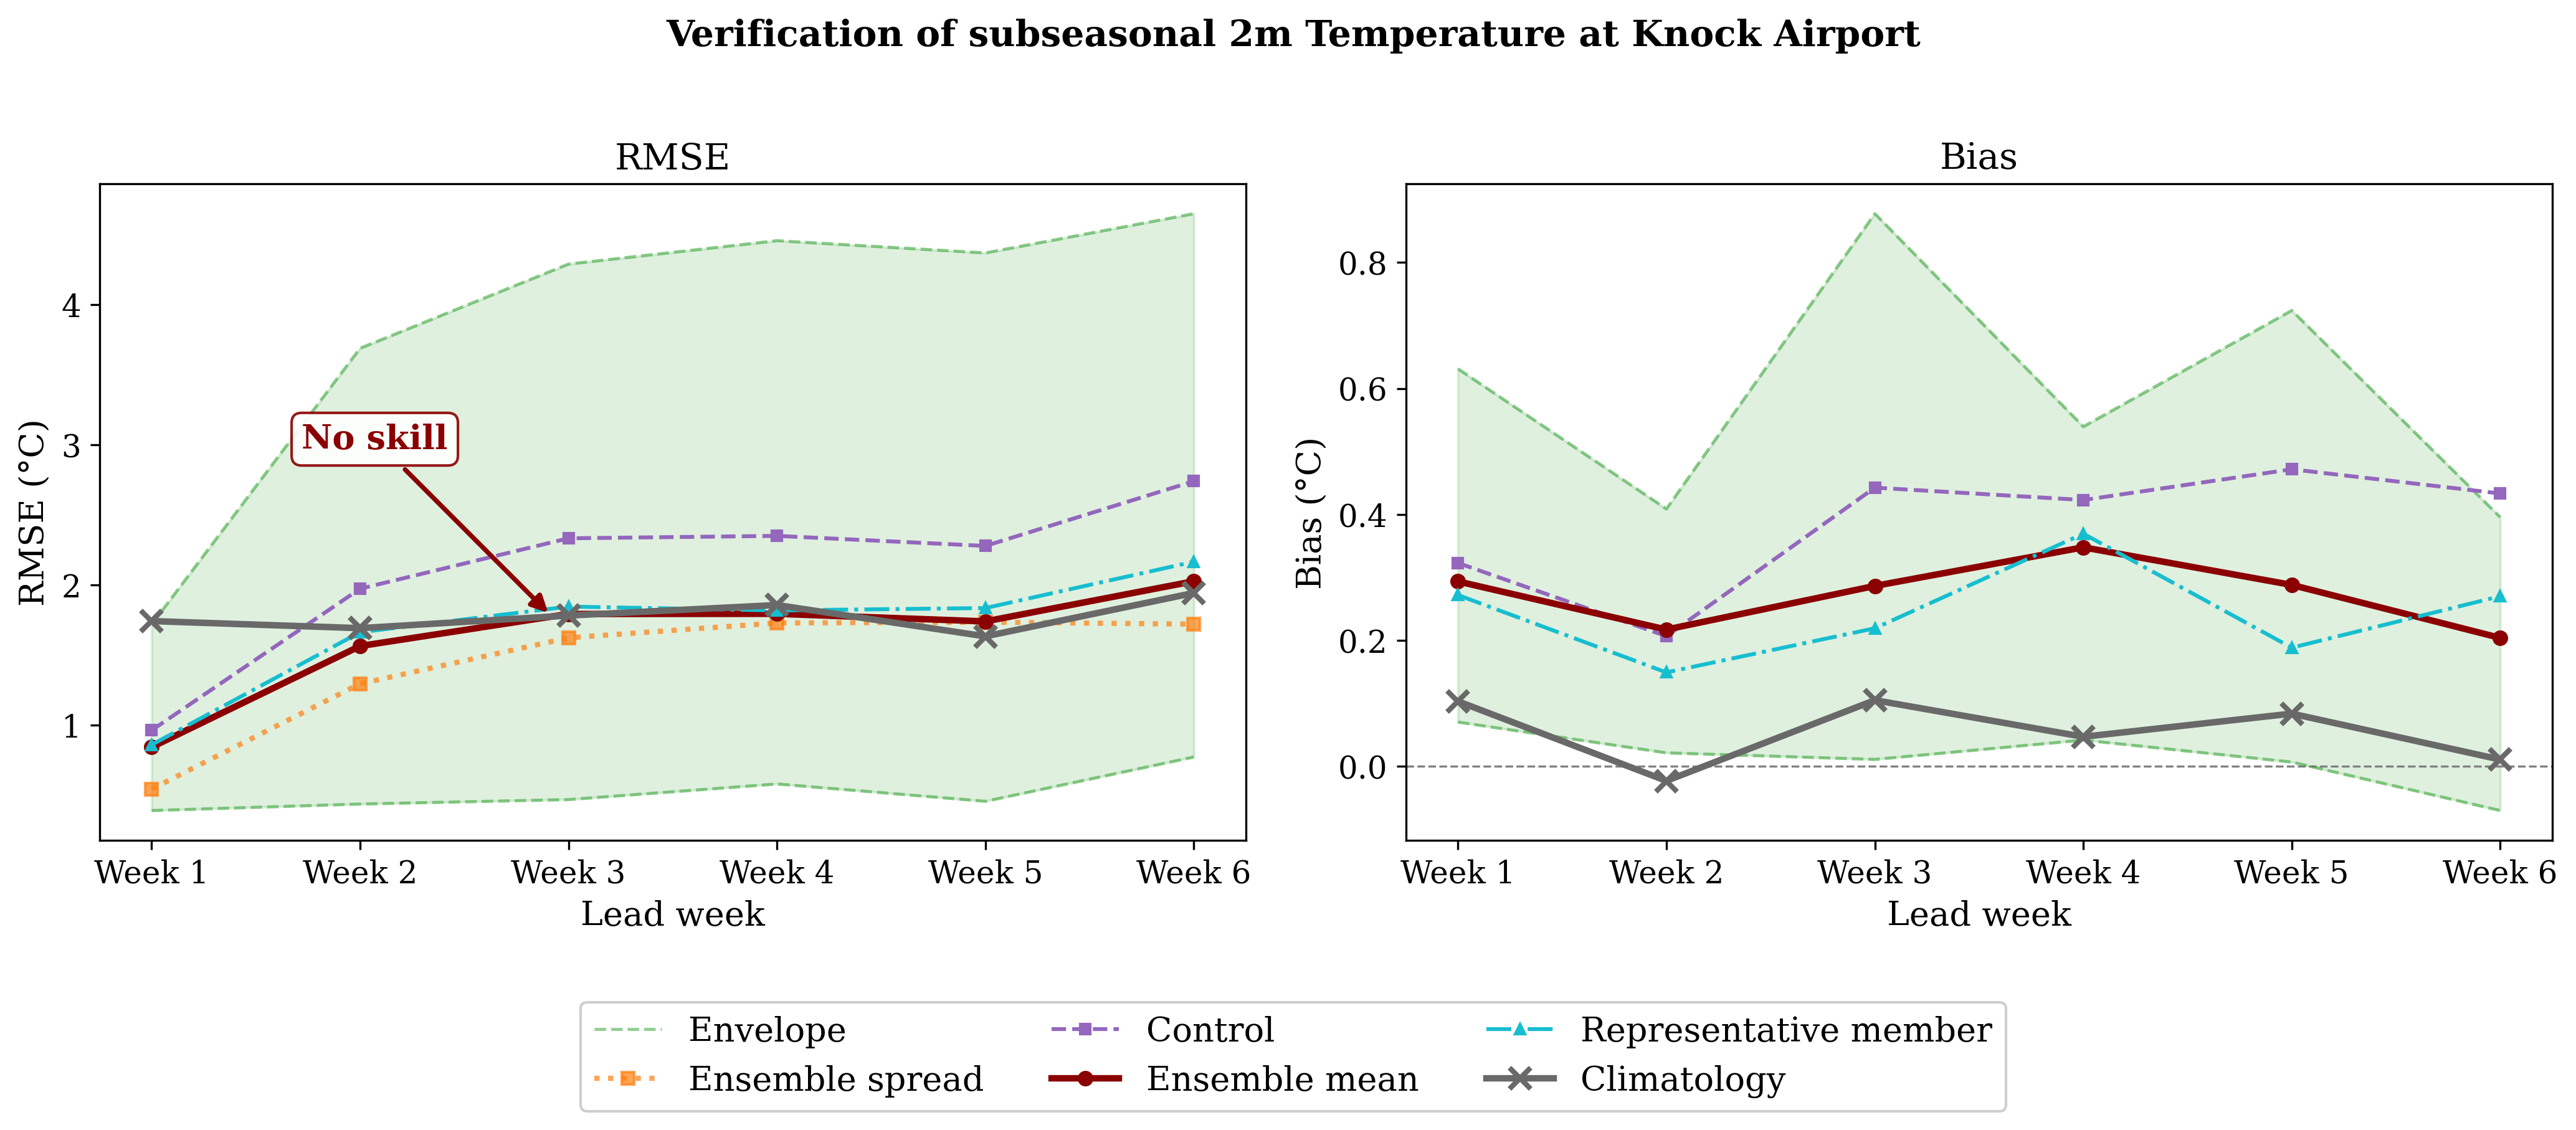
\includegraphics[width=\textwidth, height=0.80\textheight, keepaspectratio]{slide_rmse_bias_t2m_hly4935.png}
        \end{column}

    \end{columns}

\end{frame}

% Spatial RMSE
\begin{frame}{Spatial RMSE}

    \begin{columns}[c, totalwidth=\textwidth]

        \begin{column}{\textwidth}
            \centering
            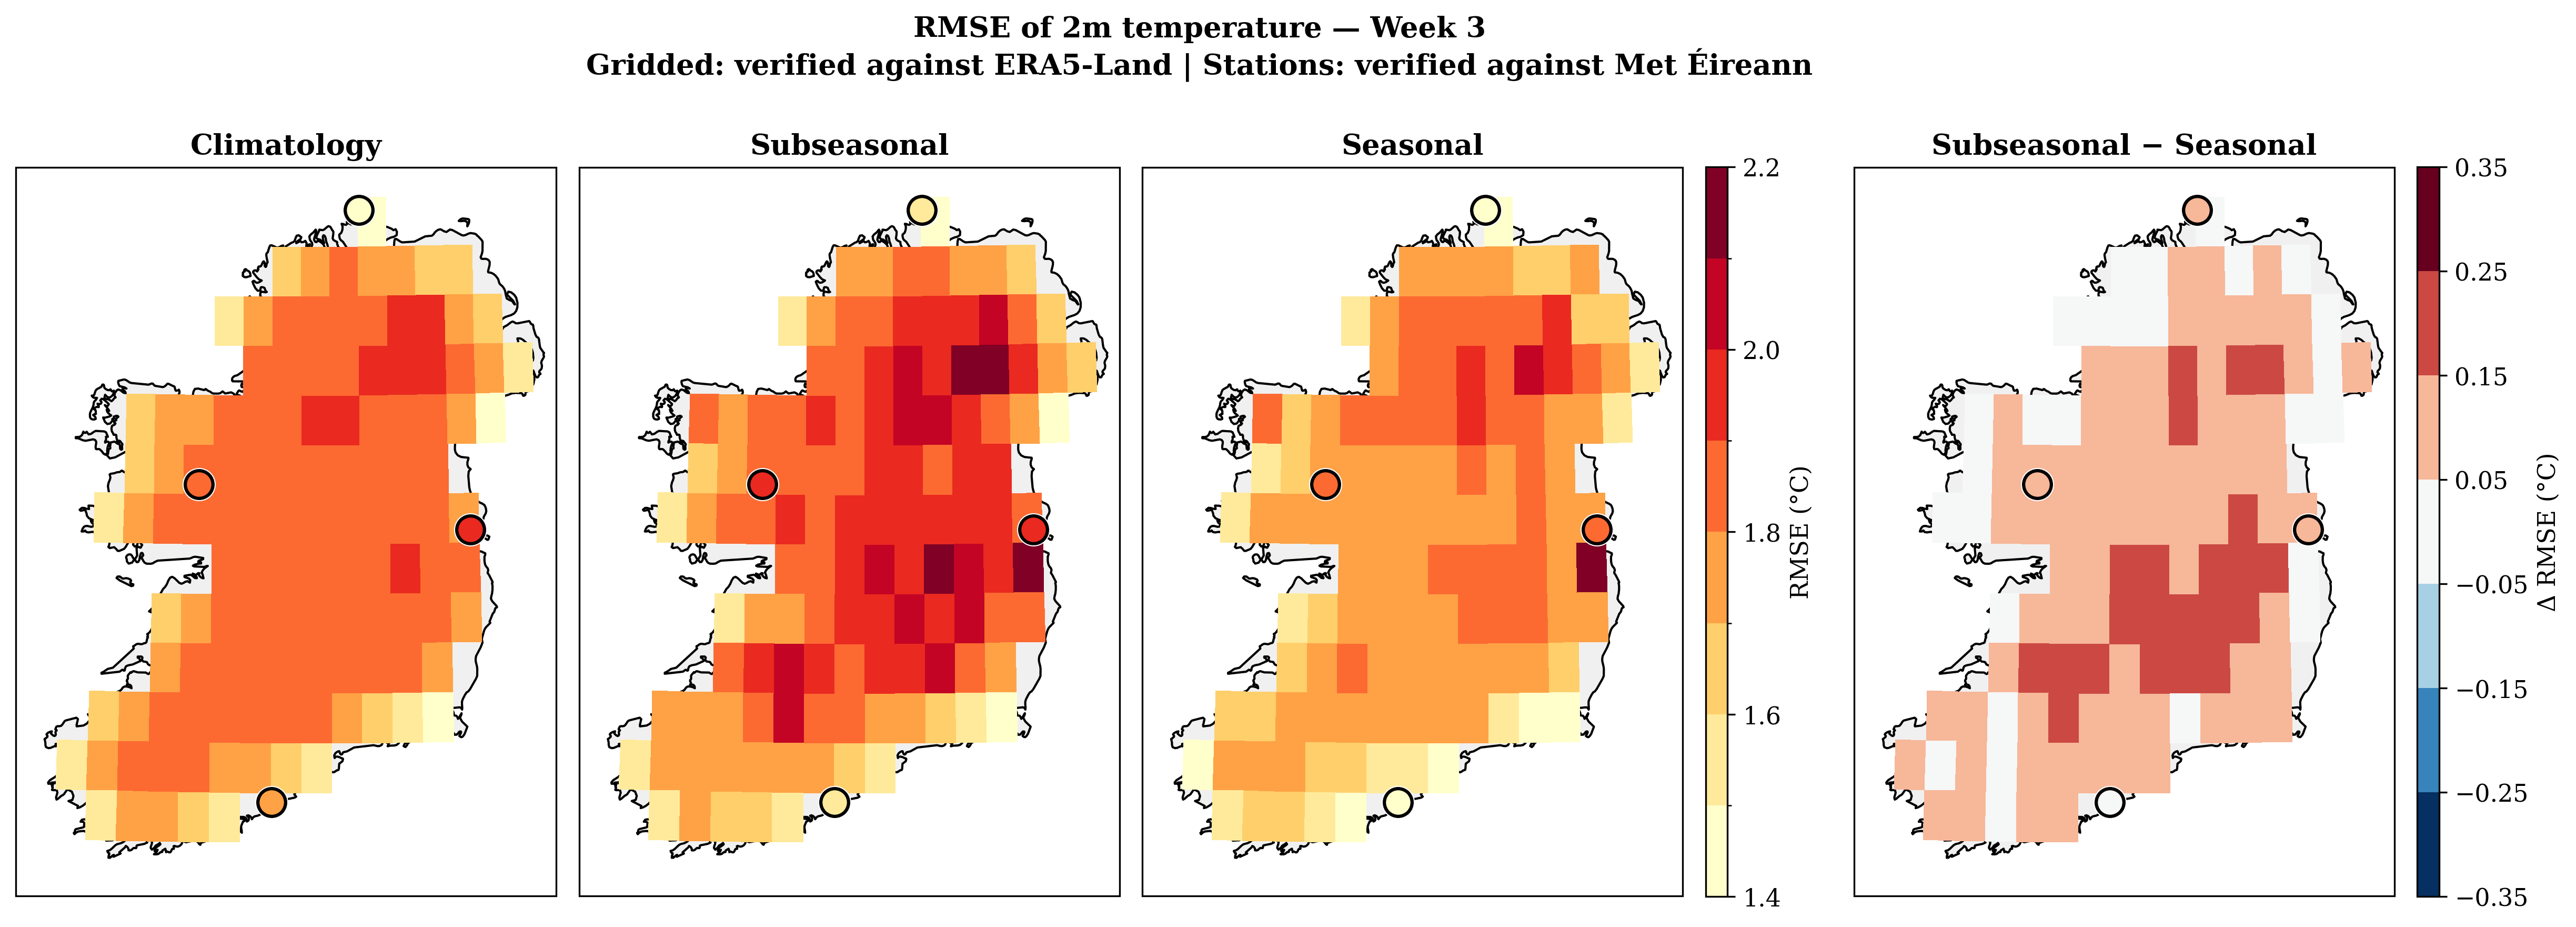
\includegraphics[width=\textwidth, height=0.85\textheight, keepaspectratio]{consolidation_spatial_rmse_4panel.png}
        \end{column}

    \end{columns}

\end{frame}

% Spatial Skill Score
\begin{frame}{Spatial Skill Score}

    \vspace{-0.5em}
    \begin{columns}[c, totalwidth=\textwidth]

        \begin{column}{0.72\textwidth}
            \centering
            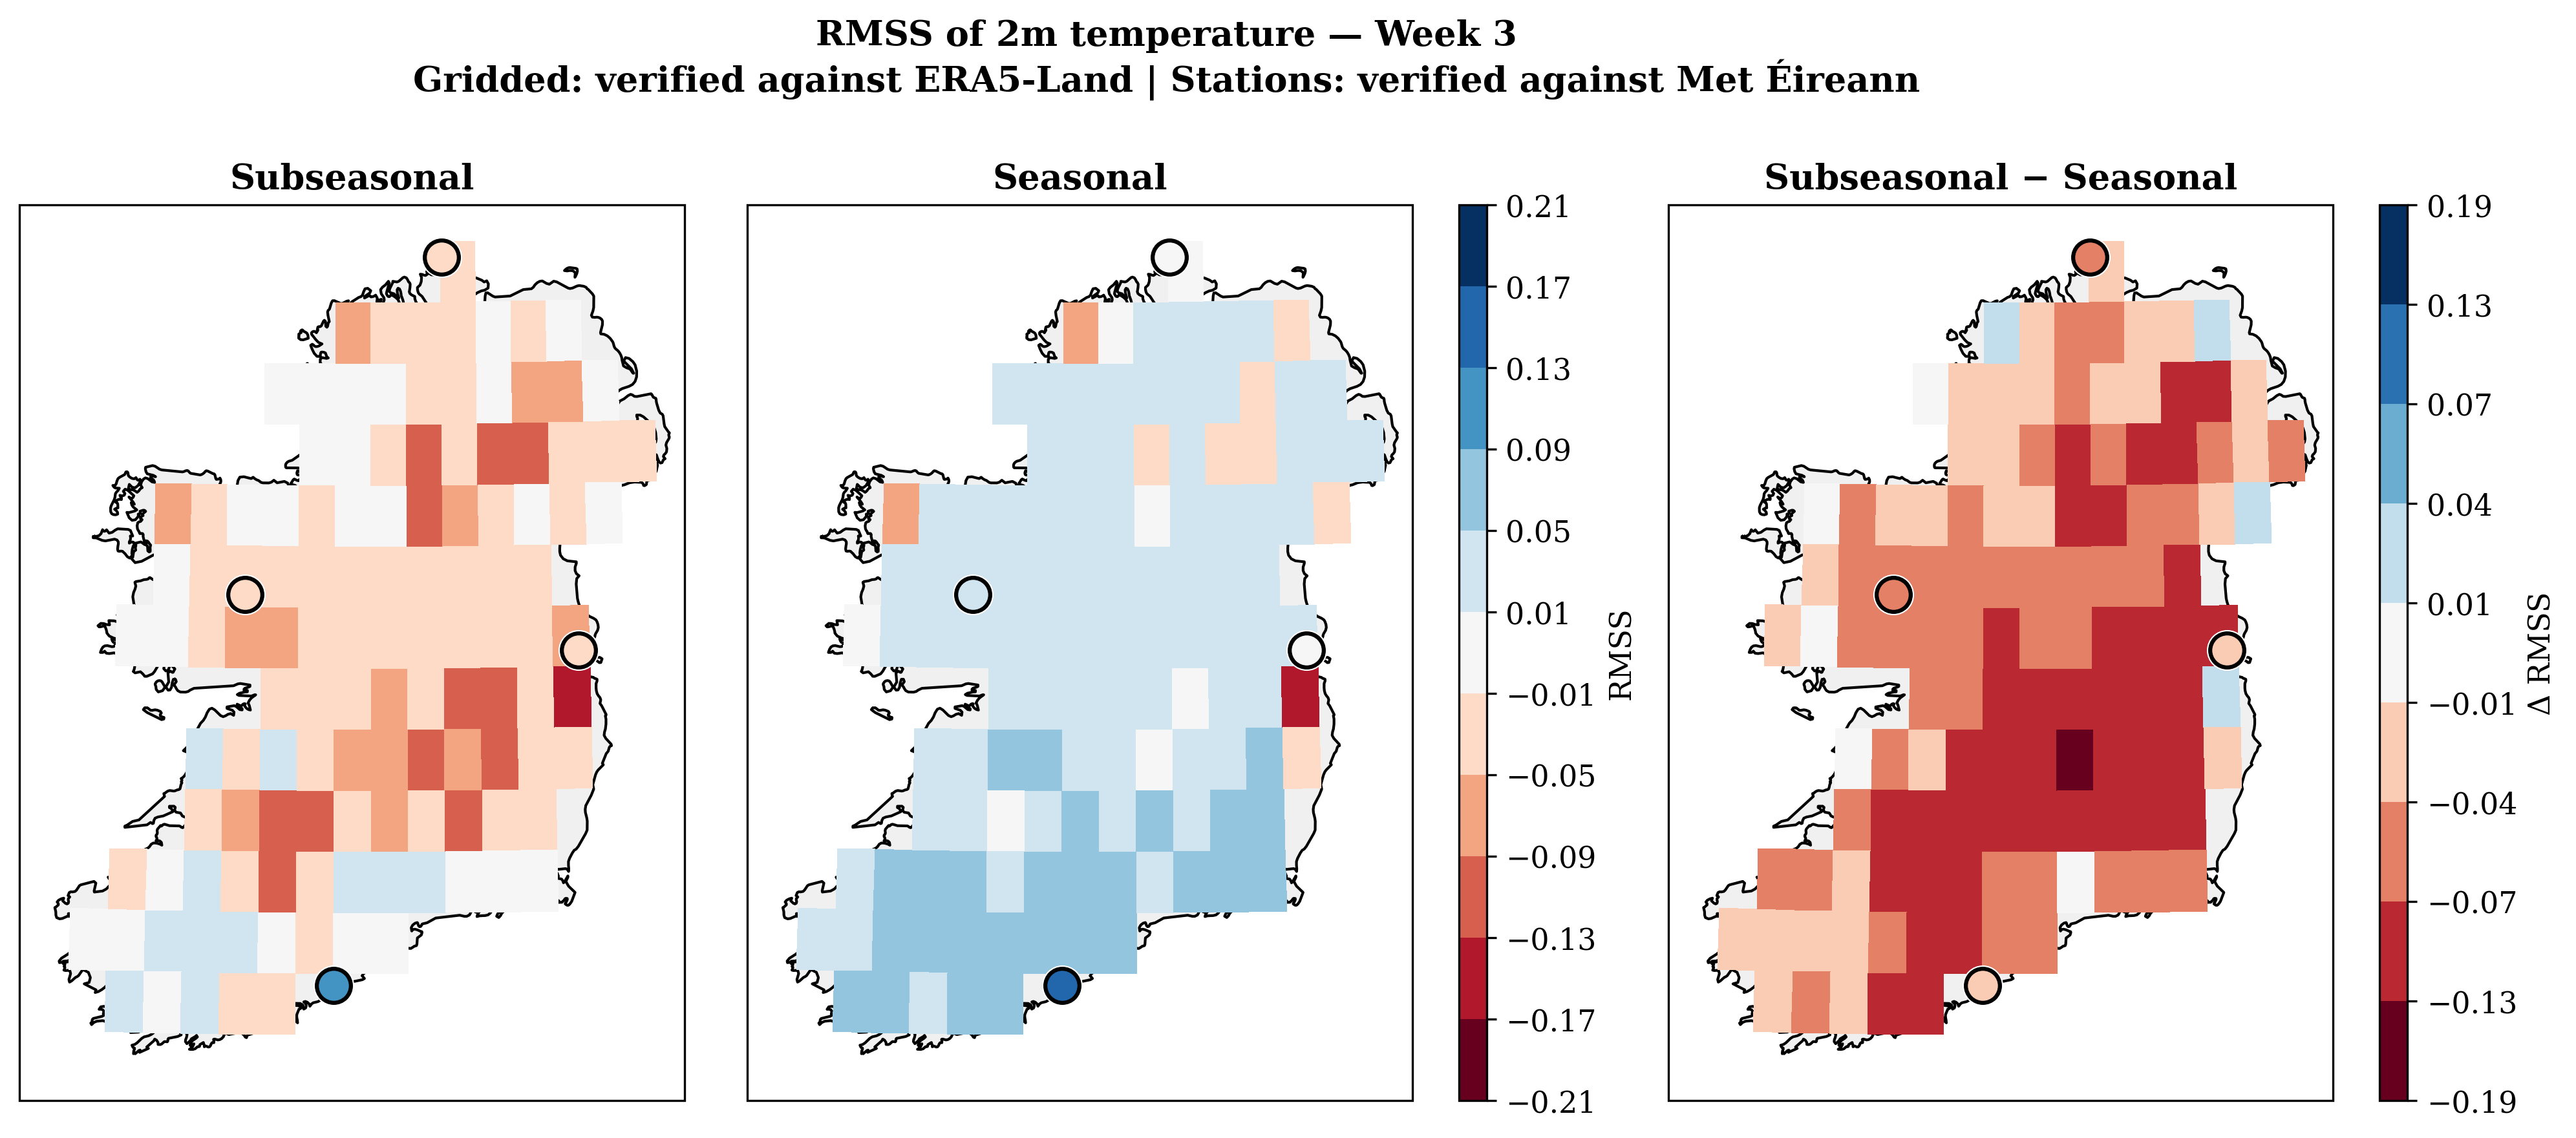
\includegraphics[width=\textwidth, height=0.80\textheight, keepaspectratio]{consolidation_spatial_rmss_3panel.png}
        \end{column}

        \begin{column}{0.26\textwidth}
            \vspace{1em}
            \begin{block}{\small RMSS}
            \small
            \[
                \text{RMSS} = 1 - \frac{\text{RMSE}_{\text{fc}}}{\text{RMSE}_{\text{clim}}}
            \]
            \vspace{0.3em}

            \textbf{RMSS $> 0$}: forecast beats climatology\\[0.3em]
            \textbf{RMSS $= 0$}: no skill\\[0.3em]
            \textbf{RMSS $< 0$}: worse than climatology
            \end{block}
        \end{column}

    \end{columns}

\end{frame}

% Venn diagram
\begin{frame}{Where the Literature Review Sits}

    \centering
    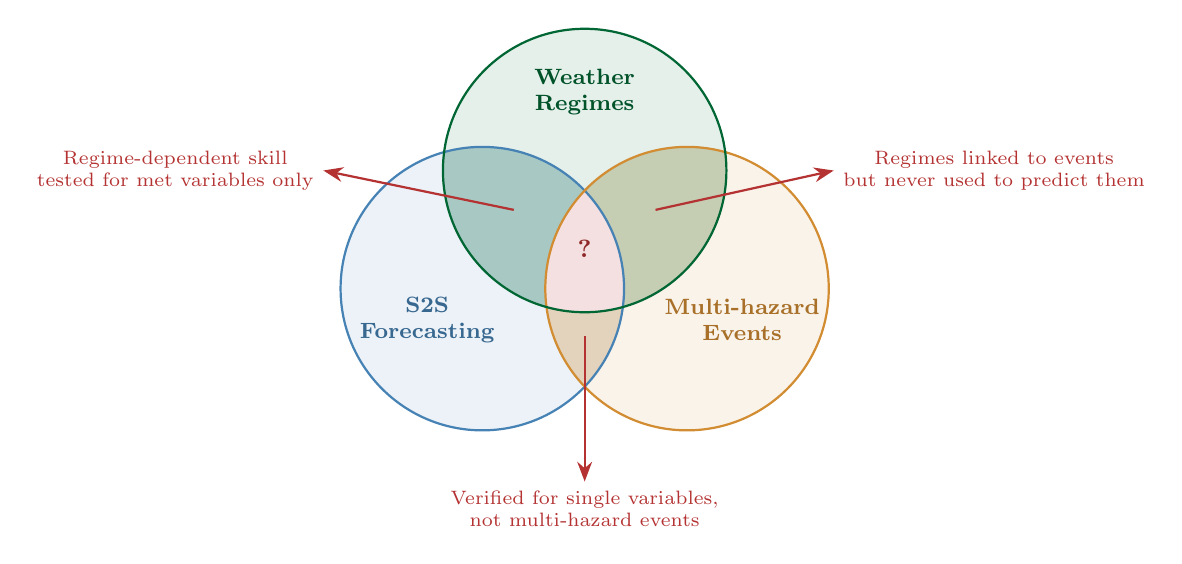
\begin{tikzpicture}
    \def\r{1.8}

    \fill[vennblue!10] (-1.3,0) circle (\r);
    \fill[vennorange!10] ( 1.3,0) circle (\r);
    \fill[ucdgreen!10] (0,1.5) circle (\r);

    \begin{scope}
      \clip (-1.3,0) circle (\r);
      \clip ( 1.3,0) circle (\r);
      \fill[vennblue!25!vennorange, opacity=0.3] (-3,-3) rectangle (3,3);
    \end{scope}
    \begin{scope}
      \clip (-1.3,0) circle (\r);
      \clip (0,1.5) circle (\r);
      \fill[vennblue!40!ucdgreen, opacity=0.3] (-3,-3) rectangle (3,3);
    \end{scope}
    \begin{scope}
      \clip ( 1.3,0) circle (\r);
      \clip (0,1.5) circle (\r);
      \fill[ucdgreen!40!vennorange, opacity=0.3] (-3,-3) rectangle (3,3);
    \end{scope}

    \begin{scope}
      \clip (-1.3,0) circle (\r);
      \clip ( 1.3,0) circle (\r);
      \clip (0,1.5) circle (\r);
      \fill[gapred!15] (-3,-3) rectangle (3,3);
    \end{scope}

    \draw[vennblue, thick] (-1.3,0) circle (\r);
    \draw[vennorange, thick] ( 1.3,0) circle (\r);
    \draw[ucdgreen, thick] (0,1.5) circle (\r);

    \node[align=center, text=vennblue!80!black, font=\footnotesize\bfseries]
        at (-2.0,-0.4) {S2S\\Forecasting};
    \node[align=center, text=vennorange!80!black, font=\footnotesize\bfseries]
        at ( 2.0,-0.4) {Multi-hazard\\Events};
    \node[align=center, text=ucdgreen!80!black, font=\footnotesize\bfseries]
        at (0,2.5) {Weather\\Regimes};

    \node[align=center, font=\small\bfseries, text=gapred!80!black]
        at (0,0.5) {?};

    \node[align=center, font=\scriptsize, text=gapred] (g1) at (0,-2.8)
         {Verified for single variables,\\not multi-hazard events};
    \draw[-{Stealth[length=2.5mm]}, thick, gapred] (0,-0.6) -- (g1.north);

    \node[align=center, font=\scriptsize, text=gapred] (g2) at (-5.2,1.5)
         {Regime-dependent skill\\tested for met variables only};
    \draw[-{Stealth[length=2.5mm]}, thick, gapred] (-0.9,1.0) -- (g2.east);

    \node[align=center, font=\scriptsize, text=gapred] (g3) at (5.2,1.5)
         {Regimes linked to events\\but never used to predict them};
    \draw[-{Stealth[length=2.5mm]}, thick, gapred] (0.9,1.0) -- (g3.west);

    \end{tikzpicture}

\end{frame}

% Variable availability
\begin{frame}{Variable Availability}

    \centering

    \newcommand{\cw}{0.6}
    \newcommand{\ch}{0.5}
    \begin{tikzpicture}[
        cell/.style={minimum width=\cw cm, minimum height=\ch cm, inner sep=0pt, outer sep=0pt},
        avail/.style={cell, fill=availgreen!80},
        deriv/.style={cell, fill=derivblue!60},
        noavail/.style={cell, fill=unavailgray!40},
        partial/.style={cell, fill=partialgreen!30},
        hdr/.style={font=\tiny\bfseries, rotate=55, anchor=south west},
        rowlbl/.style={font=\footnotesize, anchor=east},
        brace/.style={decorate, decoration={calligraphic brace, amplitude=4pt, raise=2pt},
                      thick, ucdgreen!60},
    ]

    \draw[brace] (0*\cw, 3.1) -- node[above=6pt, font=\tiny\color{gray}] {Temperature} (3*\cw, 3.1);
    \draw[brace] (3*\cw, 3.1) -- node[above=6pt, font=\tiny\color{gray}] {Precip.} (4*\cw, 3.1);
    \draw[brace] (4*\cw, 3.1) -- node[above=6pt, font=\tiny\color{gray}] {Wind} (7*\cw, 3.1);
    \draw[brace] (7*\cw, 3.1) -- node[above=6pt, font=\tiny\color{gray}] {Humid.} (8*\cw, 3.1);
    \draw[brace] (8*\cw, 3.1) -- node[above=6pt, font=\tiny\color{gray}] {Radiation} (12*\cw, 3.1);
    \draw[brace] (12*\cw, 3.1) -- node[above=6pt, font=\tiny\color{gray}] {Heat flux} (14*\cw, 3.1);
    \draw[brace] (14*\cw, 3.1) -- node[above=6pt, font=\tiny\color{gray}] {Pressure} (16*\cw, 3.1);
    \draw[brace] (16*\cw, 3.1) -- node[above=6pt, font=\tiny\color{gray}] {Cloud} (18*\cw, 3.1);
    \draw[brace] (18*\cw, 3.1) -- node[above=6pt, font=\tiny\color{gray}] {Other} (20*\cw, 3.1);

    \def\cols{t2m/0, tmax/1, tmin/2, tp/3, u10/4, v10/5, ws10/6, d2m/7, ssrd/8, strd/9, ssr/10, str/11, slhf/12, sshf/13, msl/14, sp/15, tcc/16, sun/17, snow/18, evap/19}

    \foreach \name/\col in \cols {
        \node[hdr] at (\col*\cw+0.08, 2.3) {\name};
    }

    \node[rowlbl] at (-0.2, 2.0) {Seasonal};
    \node[rowlbl] at (-0.2, 1.45) {Subseasonal};
    \node[rowlbl] at (-0.2, 0.9) {ERA5-Land};
    \node[rowlbl] at (-0.2, 0.35) {Met \'Eireann};

    \foreach \col/\s in {0/avail, 1/avail, 2/avail, 3/avail, 4/avail, 5/avail, 6/deriv, 7/avail, 8/avail, 9/avail, 10/avail, 11/avail, 12/avail, 13/avail, 14/avail, 15/avail, 16/avail, 17/avail, 18/avail, 19/avail} {
        \node[\s] at (\col*\cw+\cw/2, 2.0) {};
    }

    \foreach \col/\s in {0/avail, 1/avail, 2/avail, 3/avail, 4/avail, 5/avail, 6/deriv, 7/avail, 8/avail, 9/avail, 10/avail, 11/avail, 12/avail, 13/avail, 14/avail, 15/avail, 16/avail, 17/noavail, 18/avail, 19/noavail} {
        \node[\s] at (\col*\cw+\cw/2, 1.45) {};
    }

    \foreach \col/\s in {0/avail, 1/deriv, 2/deriv, 3/avail, 4/avail, 5/avail, 6/deriv, 7/avail, 8/avail, 9/avail, 10/avail, 11/avail, 12/avail, 13/avail, 14/deriv, 15/avail, 16/noavail, 17/noavail, 18/avail, 19/avail} {
        \node[\s] at (\col*\cw+\cw/2, 0.9) {};
    }

    \foreach \col/\s in {0/avail, 1/deriv, 2/deriv, 3/avail, 4/noavail, 5/noavail, 6/avail, 7/avail, 8/noavail, 9/noavail, 10/noavail, 11/noavail, 12/noavail, 13/noavail, 14/avail, 15/noavail, 16/partial, 17/partial, 18/noavail, 19/noavail} {
        \node[\s] at (\col*\cw+\cw/2, 0.35) {};
    }

    \foreach \row in {0.35, 0.9, 1.45, 2.0} {
        \foreach \col in {0,...,19} {
            \draw[gray!20] (\col*\cw, \row-\ch/2) rectangle +(\cw, \ch);
        }
    }

    \node[font=\scriptsize, anchor=north] at (6, -0.3) {%
        \begin{tikzpicture}[baseline=-0.5ex]
            \fill[availgreen!80] (0,0) rectangle (0.25,0.25);
            \node[right, font=\scriptsize] at (0.35,0.125) {Available};
            \fill[derivblue!60] (2.3,0) rectangle (2.55,0.25);
            \node[right, font=\scriptsize] at (2.65,0.125) {Derivable};
            \fill[unavailgray!40] (4.6,0) rectangle (4.85,0.25);
            \node[right, font=\scriptsize] at (4.95,0.125) {Not available};
            \fill[partialgreen!30] (7.4,0) rectangle (7.65,0.25);
            \node[right, font=\scriptsize] at (7.75,0.125) {Partial (12 synoptic)};
        \end{tikzpicture}%
    };

    \end{tikzpicture}

\end{frame}

\end{document}
